\section{طراحی و شبیه‌سازی کنترل‌کننده برای کانال رول-پیچ-یاو}\label{roll_pitch_yaw_lqidg_section}
در بخش
\ref{quadall3}
شبیه‌سازی سه درجه آزادی استند چهارپره انجام شد. در این بخش به بررسی عملکرد چهارپره در حضور کنترل‌کننده \lr{LQIDG} پرداخته می‌شود. کنترل‌کننده \lr{LQIDG} در بخش‌های
\ref{LQIDG}
\subsection{شبیه‌سازی کنترل‌کننده به‌صورت سه کانال تک ورودی}
بررسی شده است.
 در شبیه‌سازی برای بهینه‌سازی ضرایب وزنی \lr{LQIDG} از روش بهینه‌سازی
\lr{TCACS} \cite{Karimi2010}
استفاده شده‌است.

%\begin{figure}[H]
%	\centering
%	\begin{subfigure}[H]
%		\centering
%		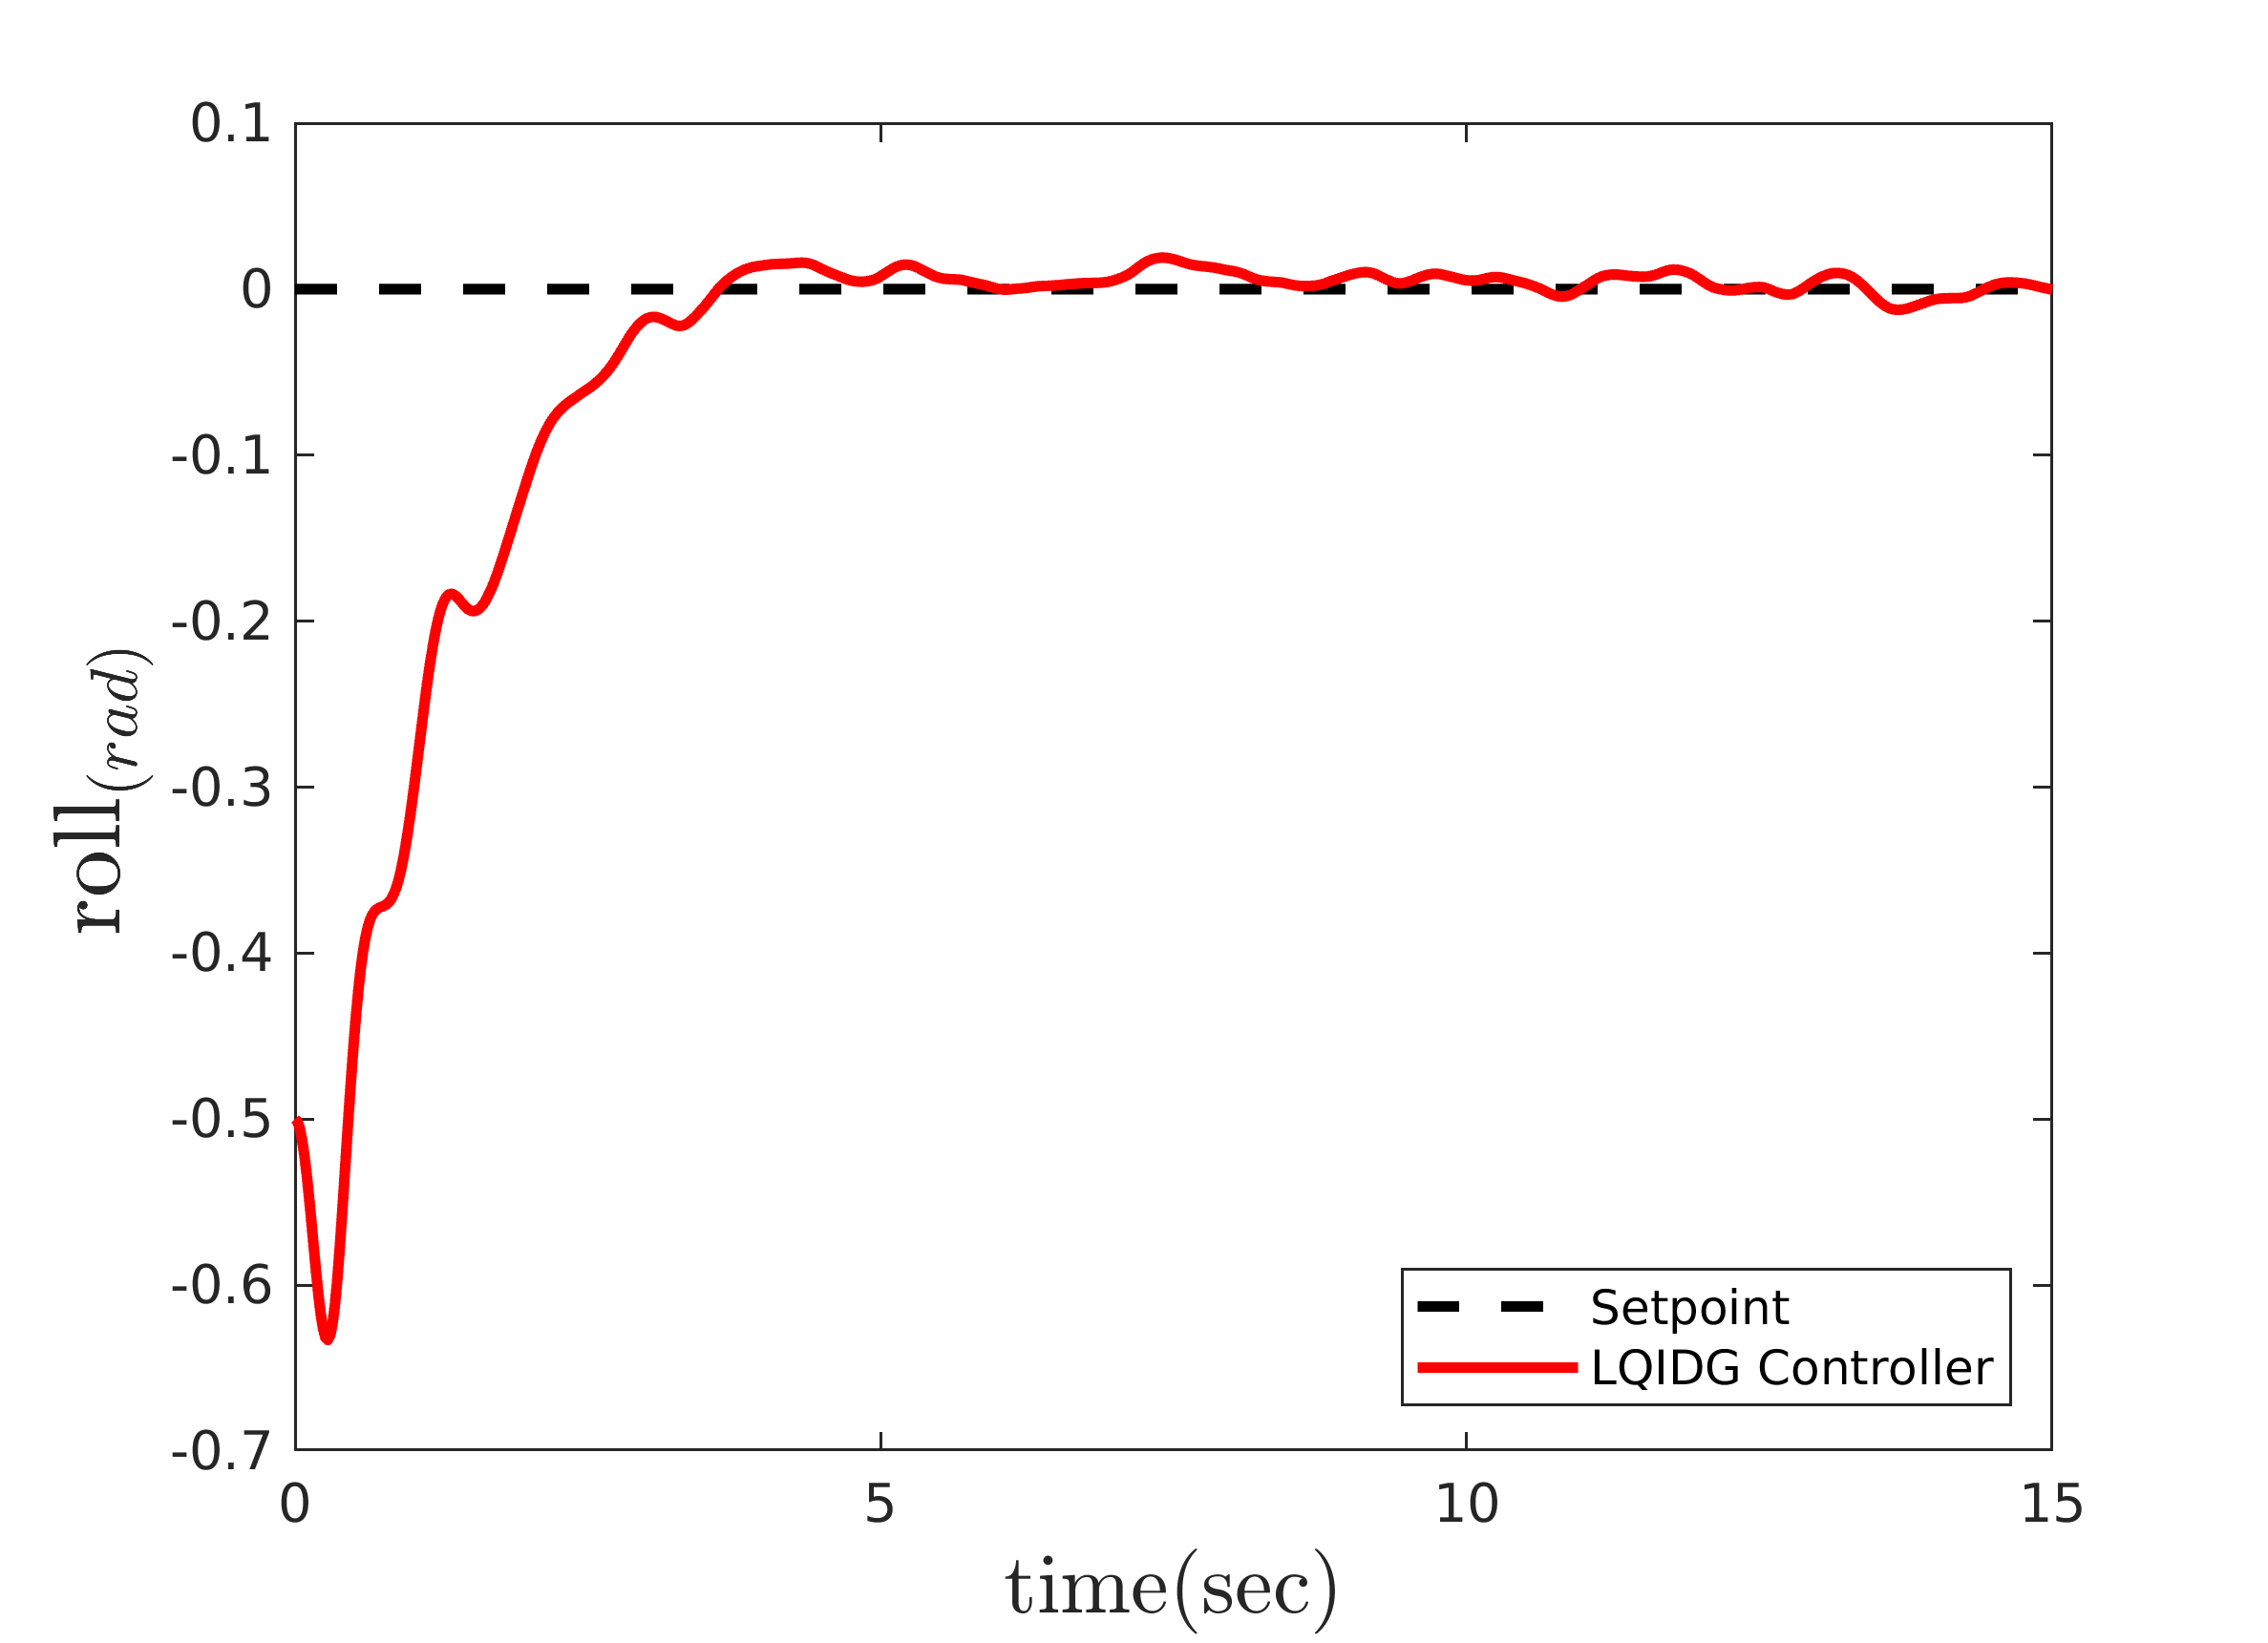
\includegraphics[width=12cm]{../Figures/MIL/LQIDG/3DOF/lqidg_roll.png}
%		\caption{تغییرات زاویه رول}
%	\end{subfigure}%
%	\begin{subfigure}
%		\centering
%		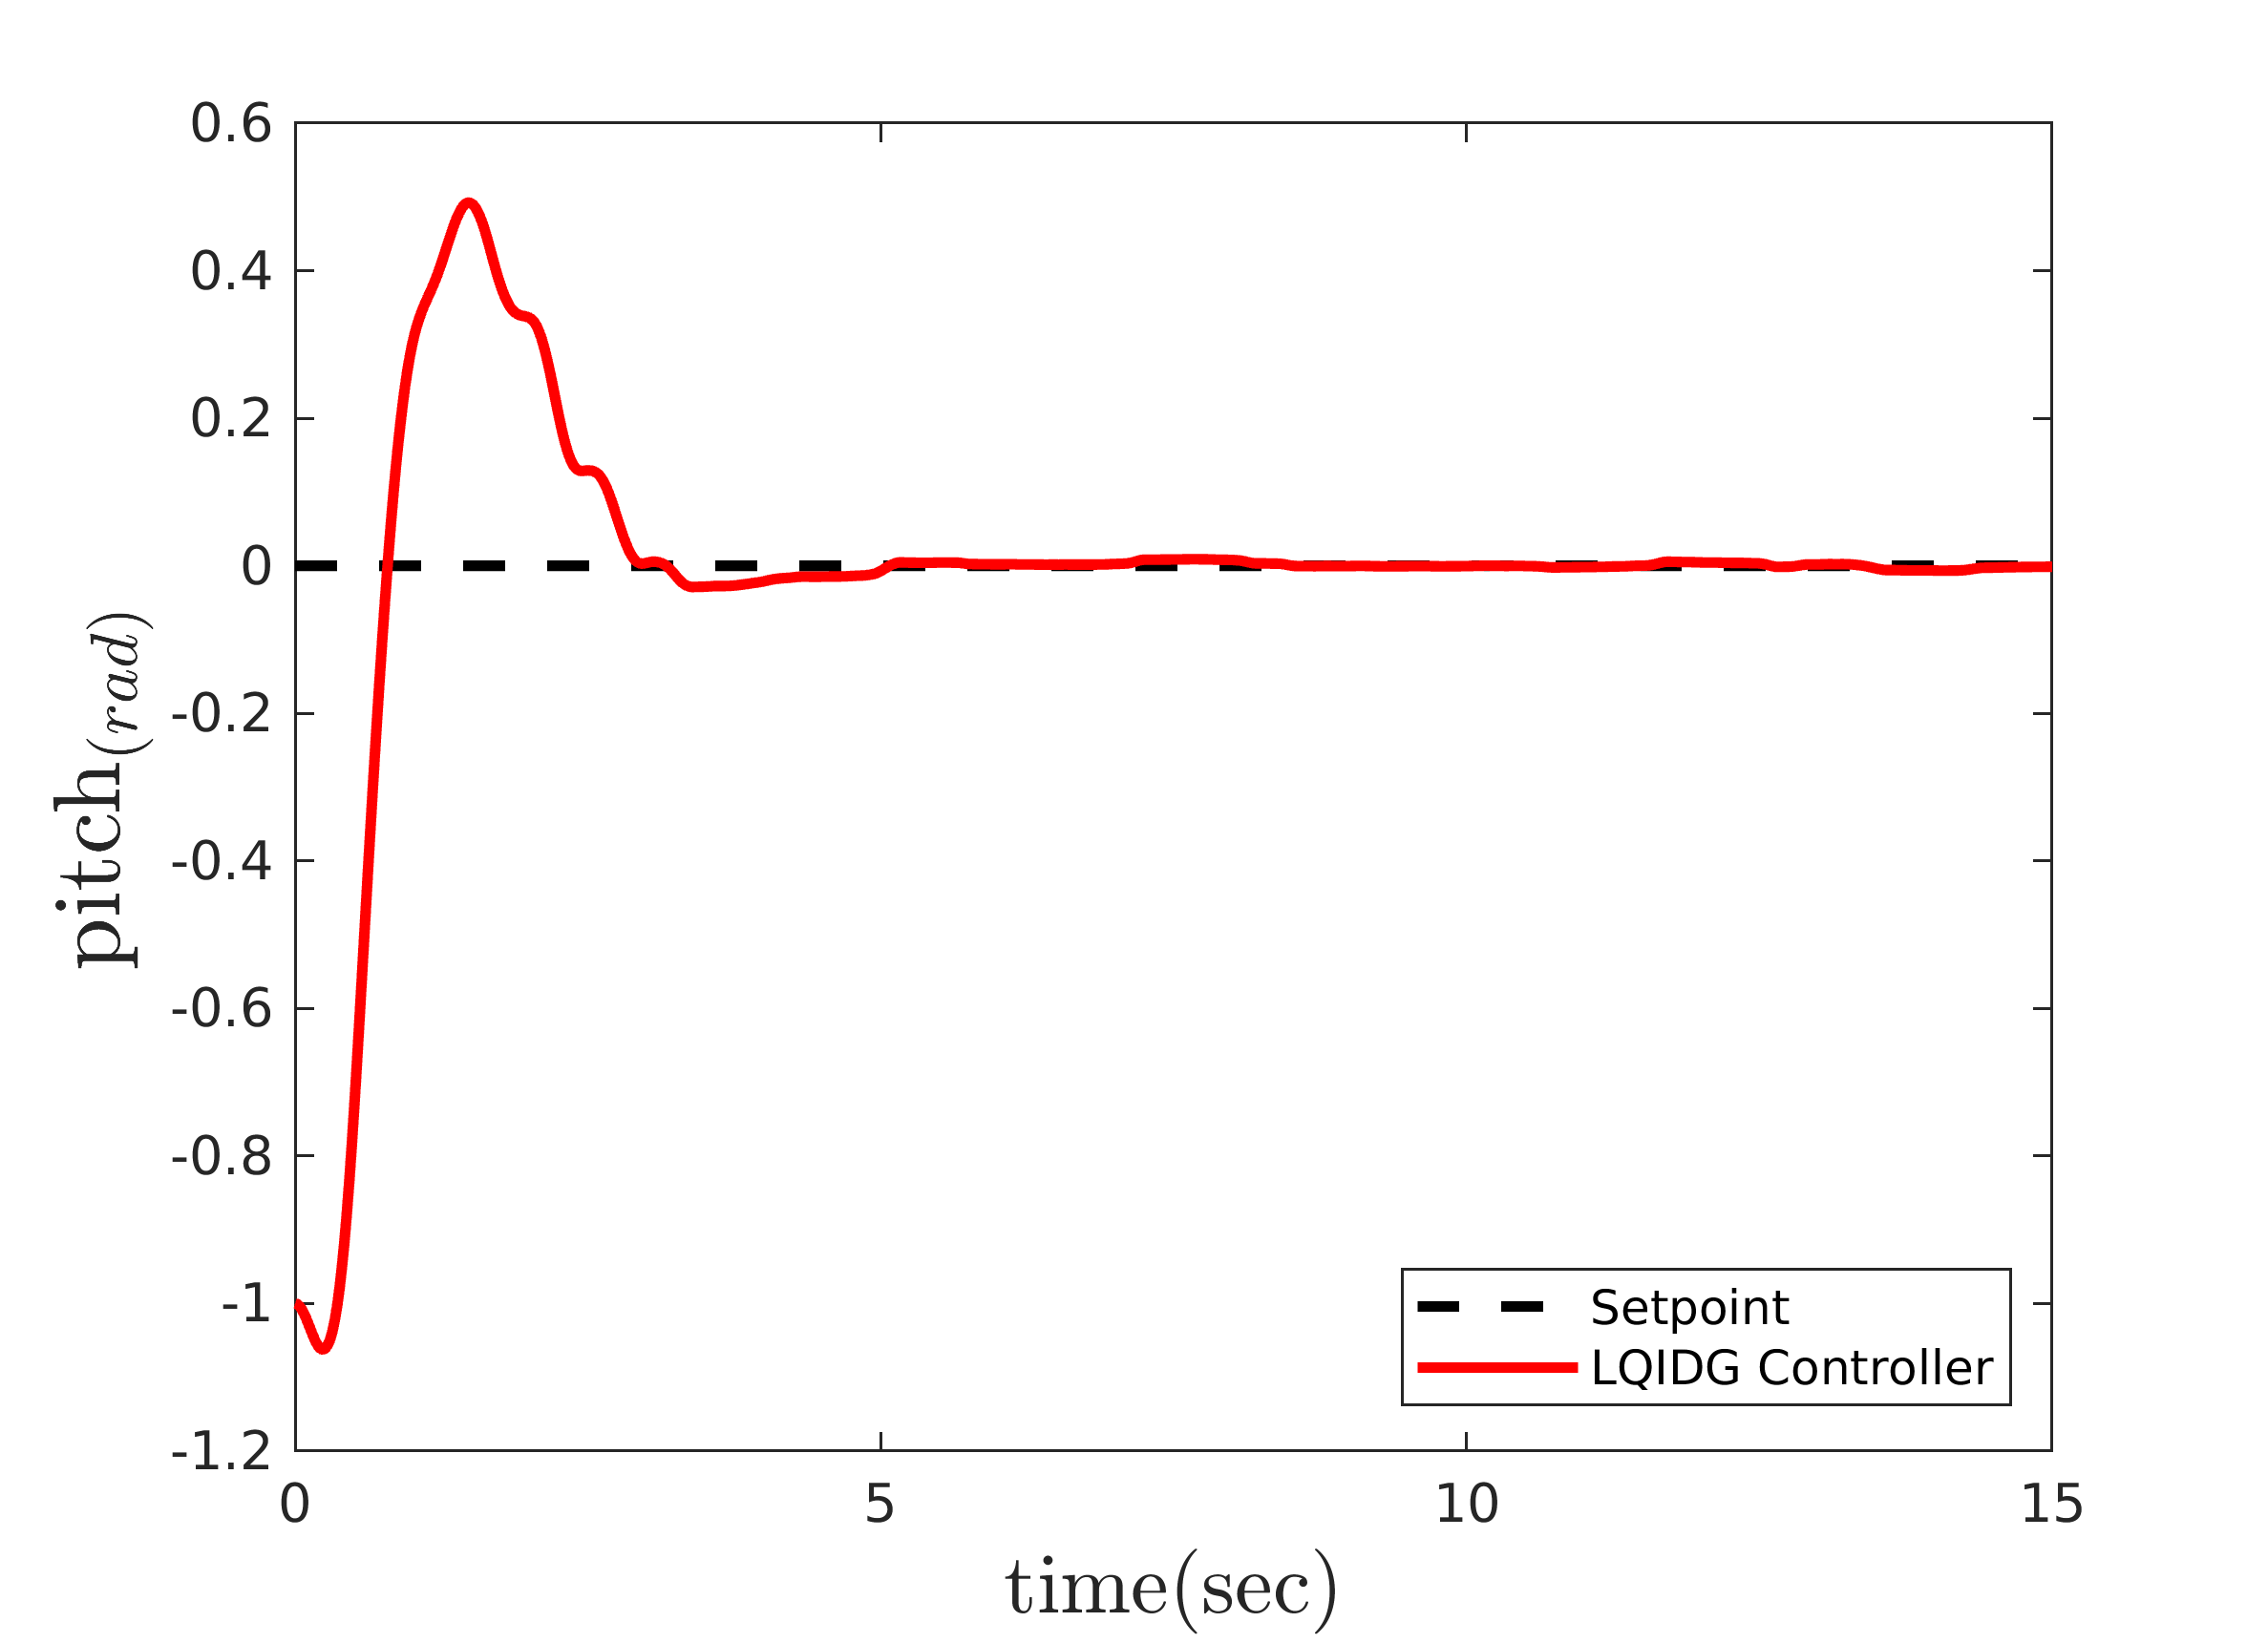
\includegraphics[width=12cm]{../Figures/MIL/LQIDG/3DOF/lqidg_pitch.png}
%		\caption{تغییرات زاویه پیچ}
%	\end{subfigure}
%	\caption{‫‪عملکرد کنترل‌کننده LQIDG در کنترل زاویه رول، پیچ و یاد (تعقیب ورودی صفر)}
%\end{figure}
%
%\begin{figure}[H]
%	\centering
%	\begin{subfigure}[H]
%		\centering
%		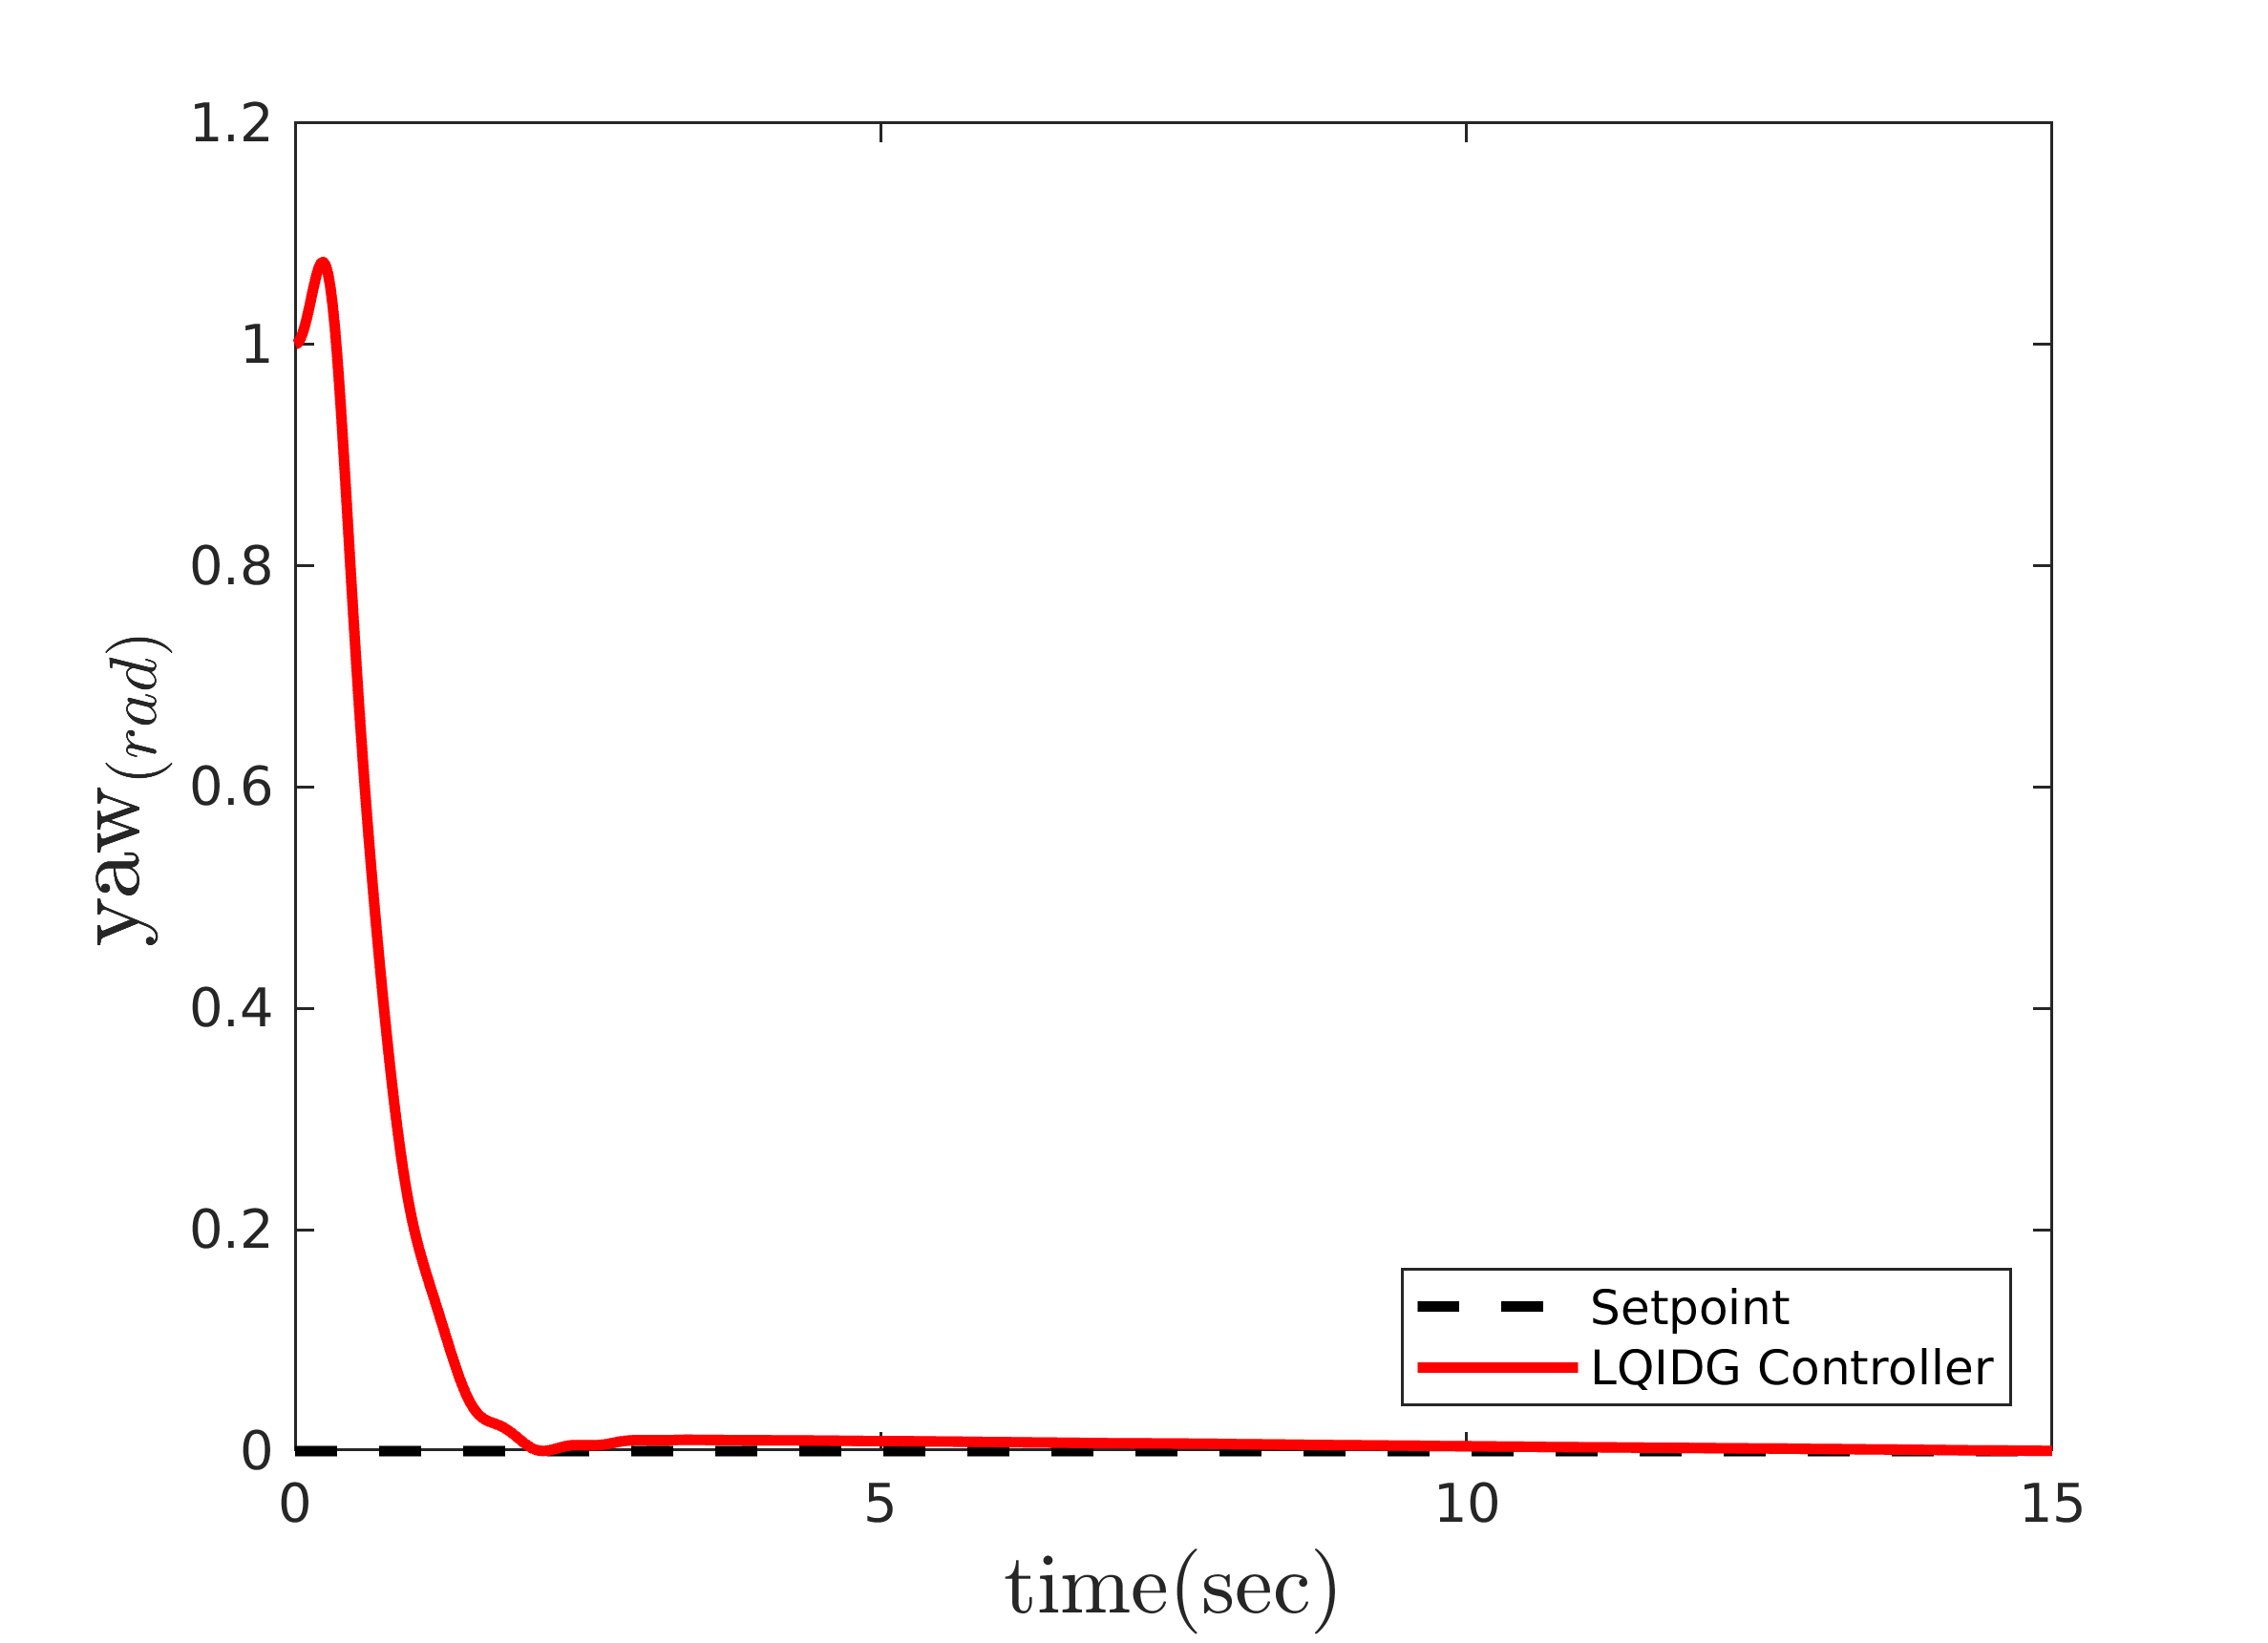
\includegraphics[width=12cm]{../Figures/MIL/LQIDG/3DOF/lqidg_yaw.png}
%		\caption{تغییرات زاویه یاو}
%	\end{subfigure}
%	\caption{‫‪عملکرد کنترل‌کننده LQIDG در کنترل زاویه رول، پیچ و یاد (تعقیب ورودی صفر)}
%\end{figure}
\begin{figure}[H]
	\centering
\subfigure[تغییرات زاویه رول]{
	\centering
	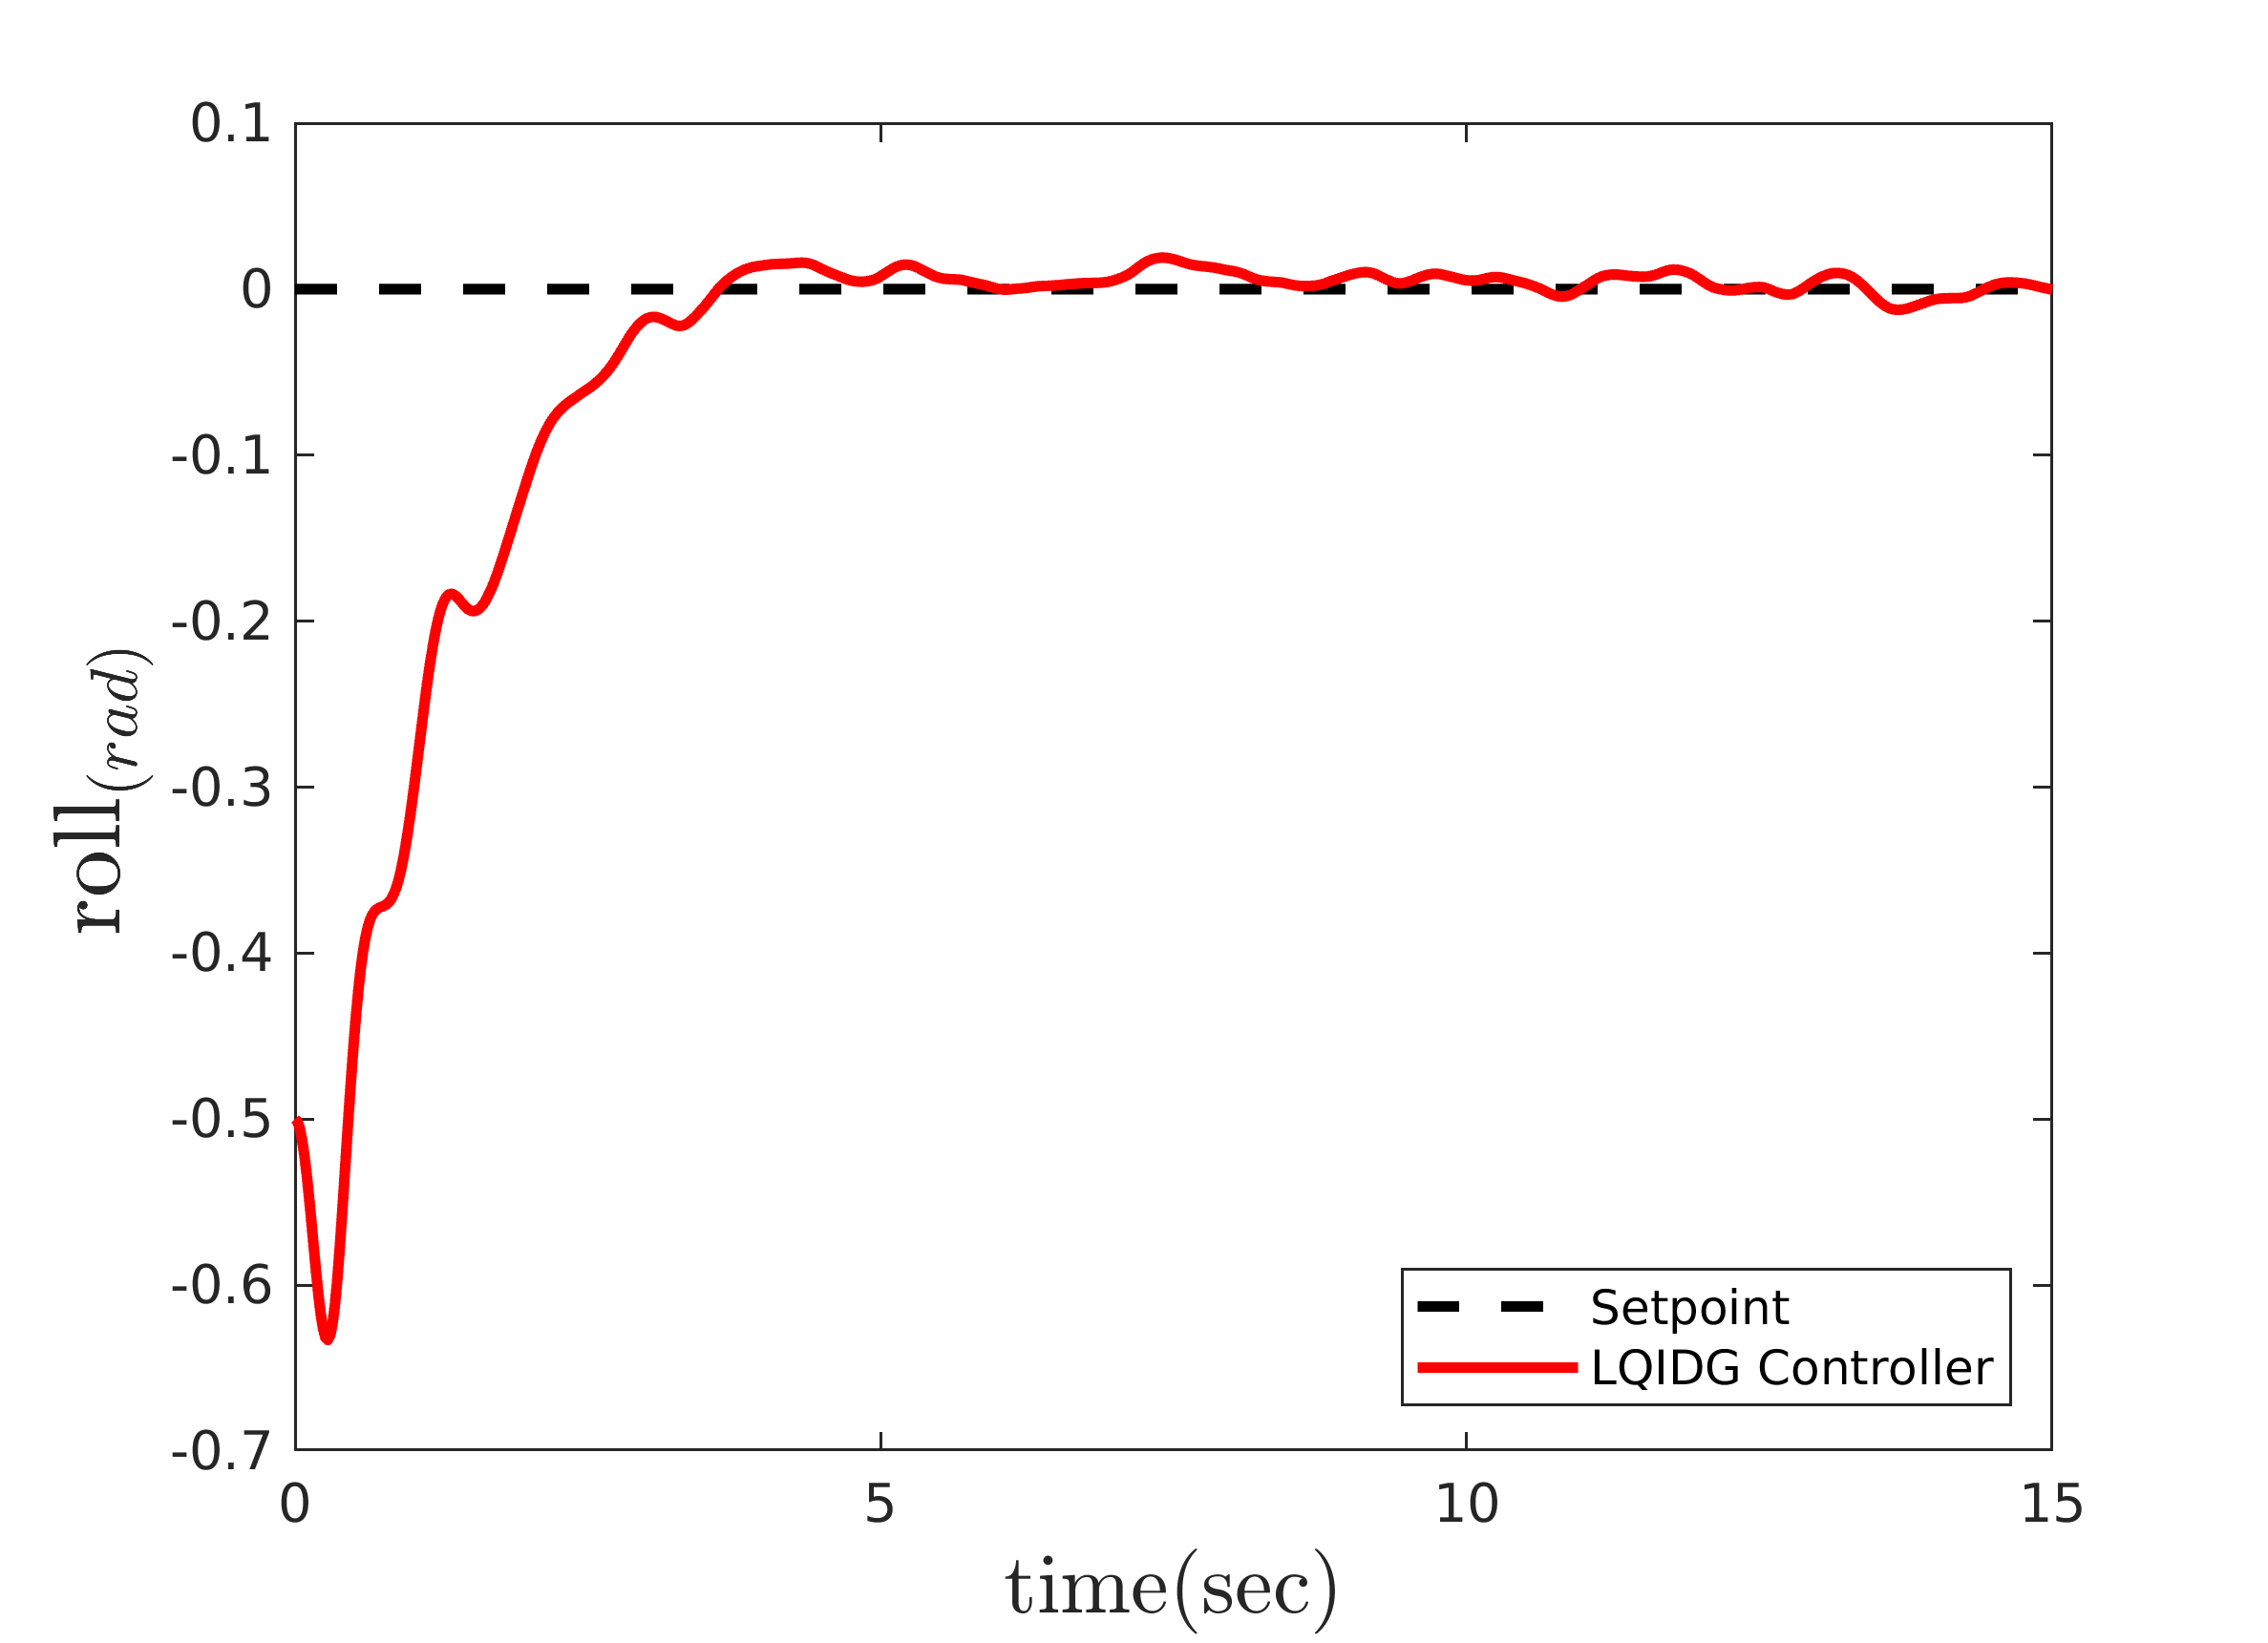
\includegraphics[width=.48\linewidth]{../Figures/MIL/LQIDG/3DOF/lqidg_roll.png}
}
\subfigure[تغییرات زاویه پیچ]{
	\centering
	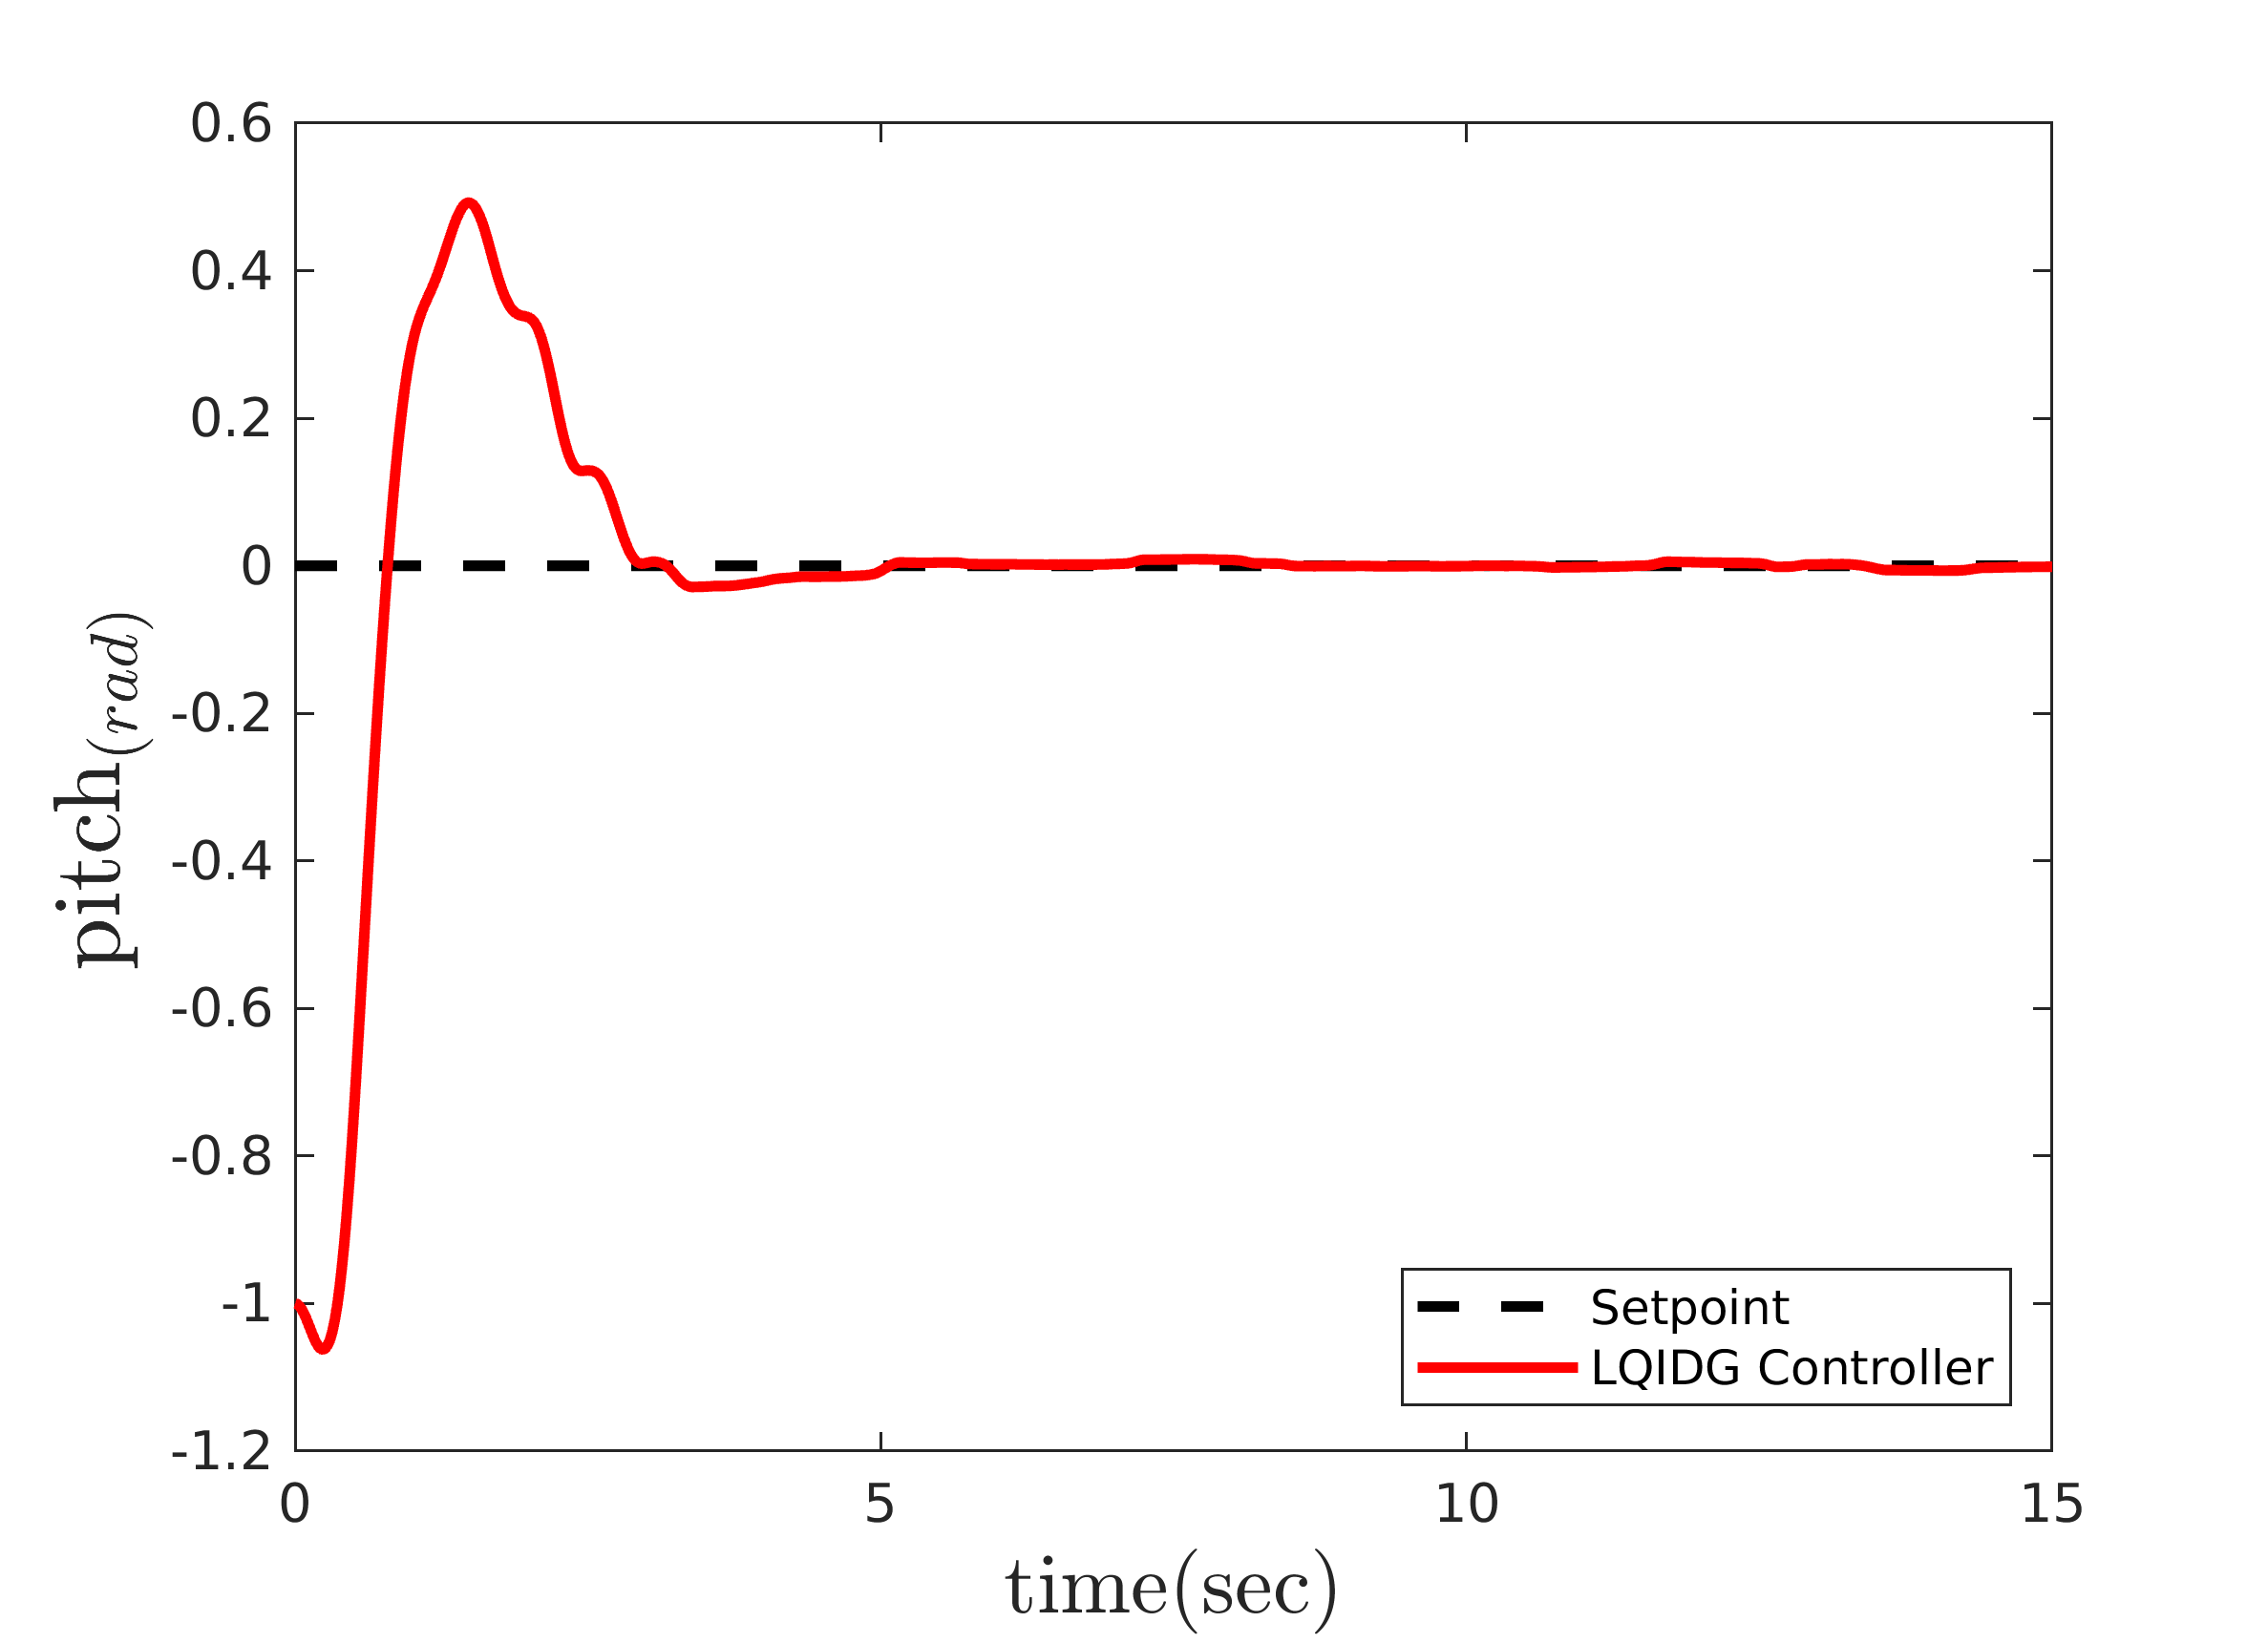
\includegraphics[width=.48\linewidth]{../Figures/MIL/LQIDG/3DOF/lqidg_pitch.png}
}
\subfigure[تغییرات زاویه یاو]{
	\centering
	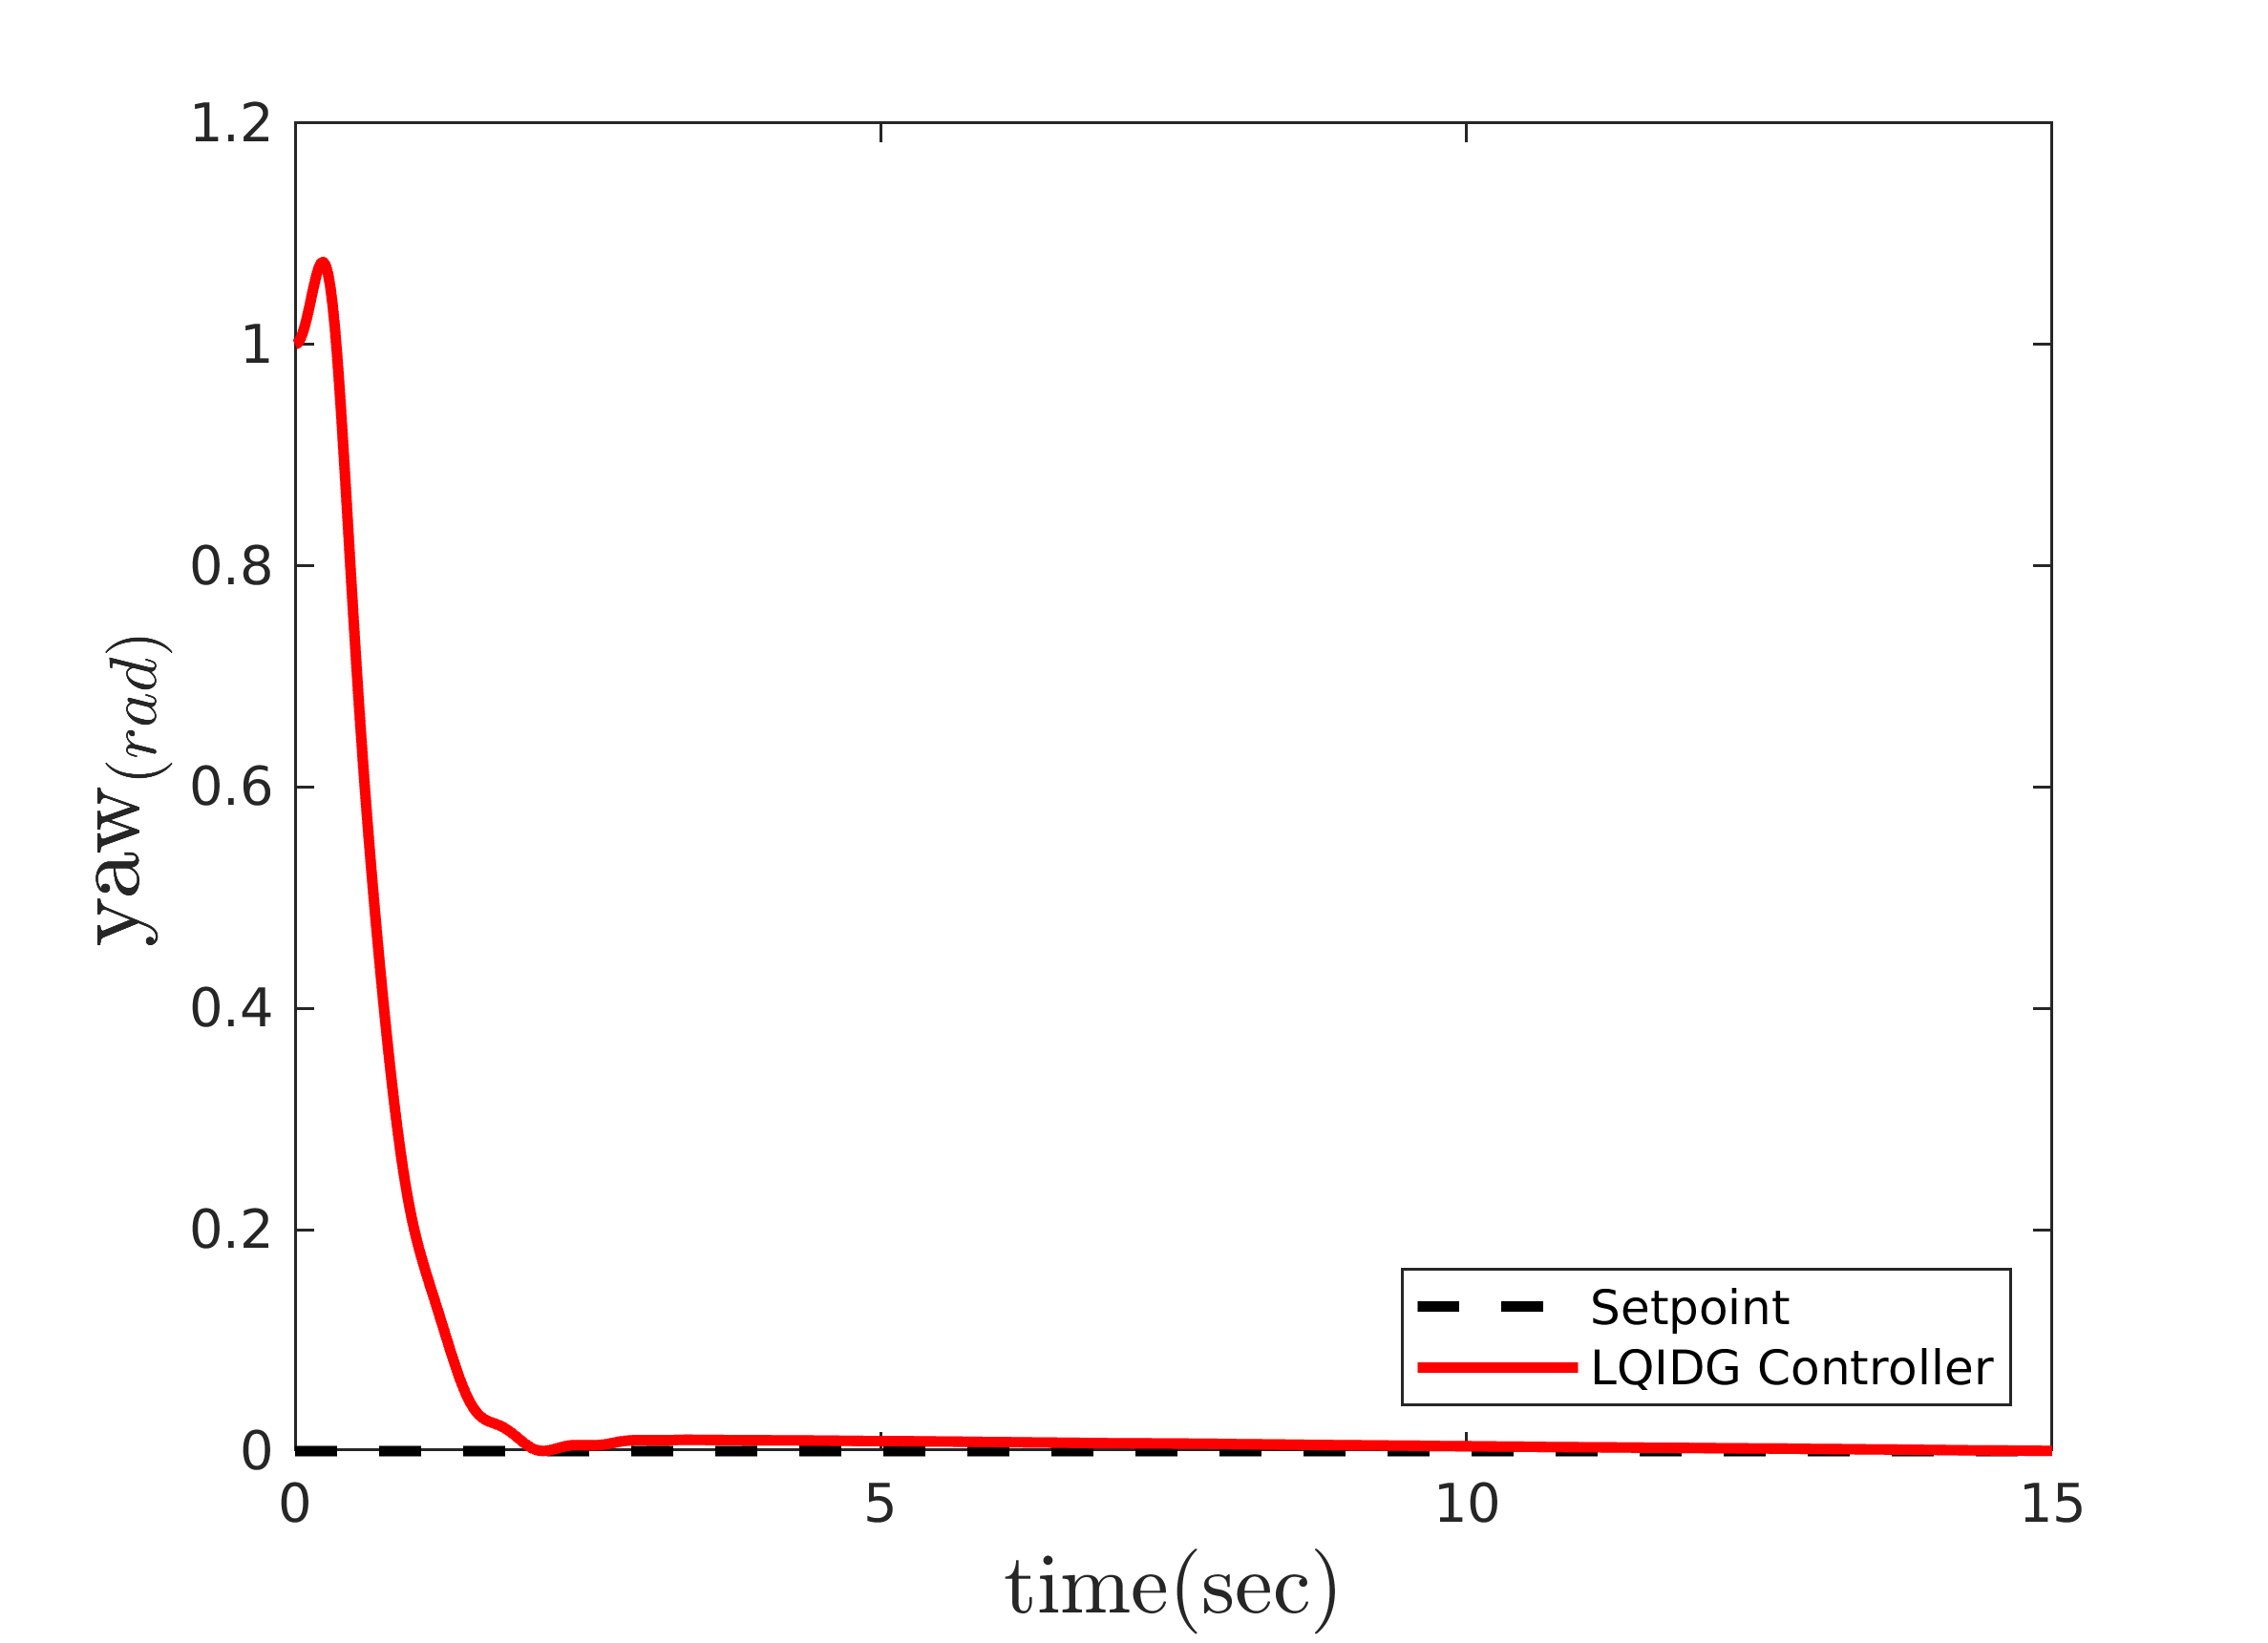
\includegraphics[width=.48\linewidth]{../Figures/MIL/LQIDG/3DOF/lqidg_yaw.png}
}
	\caption{‫‪عملکرد کنترل‌کننده \lr{LQIDG} در کنترل زاویه رول، پیچ و یاو (تعقیب ورودی صفر)}
	\label{lqidg_roll_pitch_yaw_fig_simulation}
\end{figure}


\begin{figure}[H]
	\centering
	\subfigure[موتور شماره یک]{
		\centering
		\includegraphics[width=.45\linewidth]{../Figures/MIL/LQIDG/3DOF/lqidg_roll_pitch_Omega_1.png}
	}
	\subfigure[موتور شماره دو]{
		\centering
		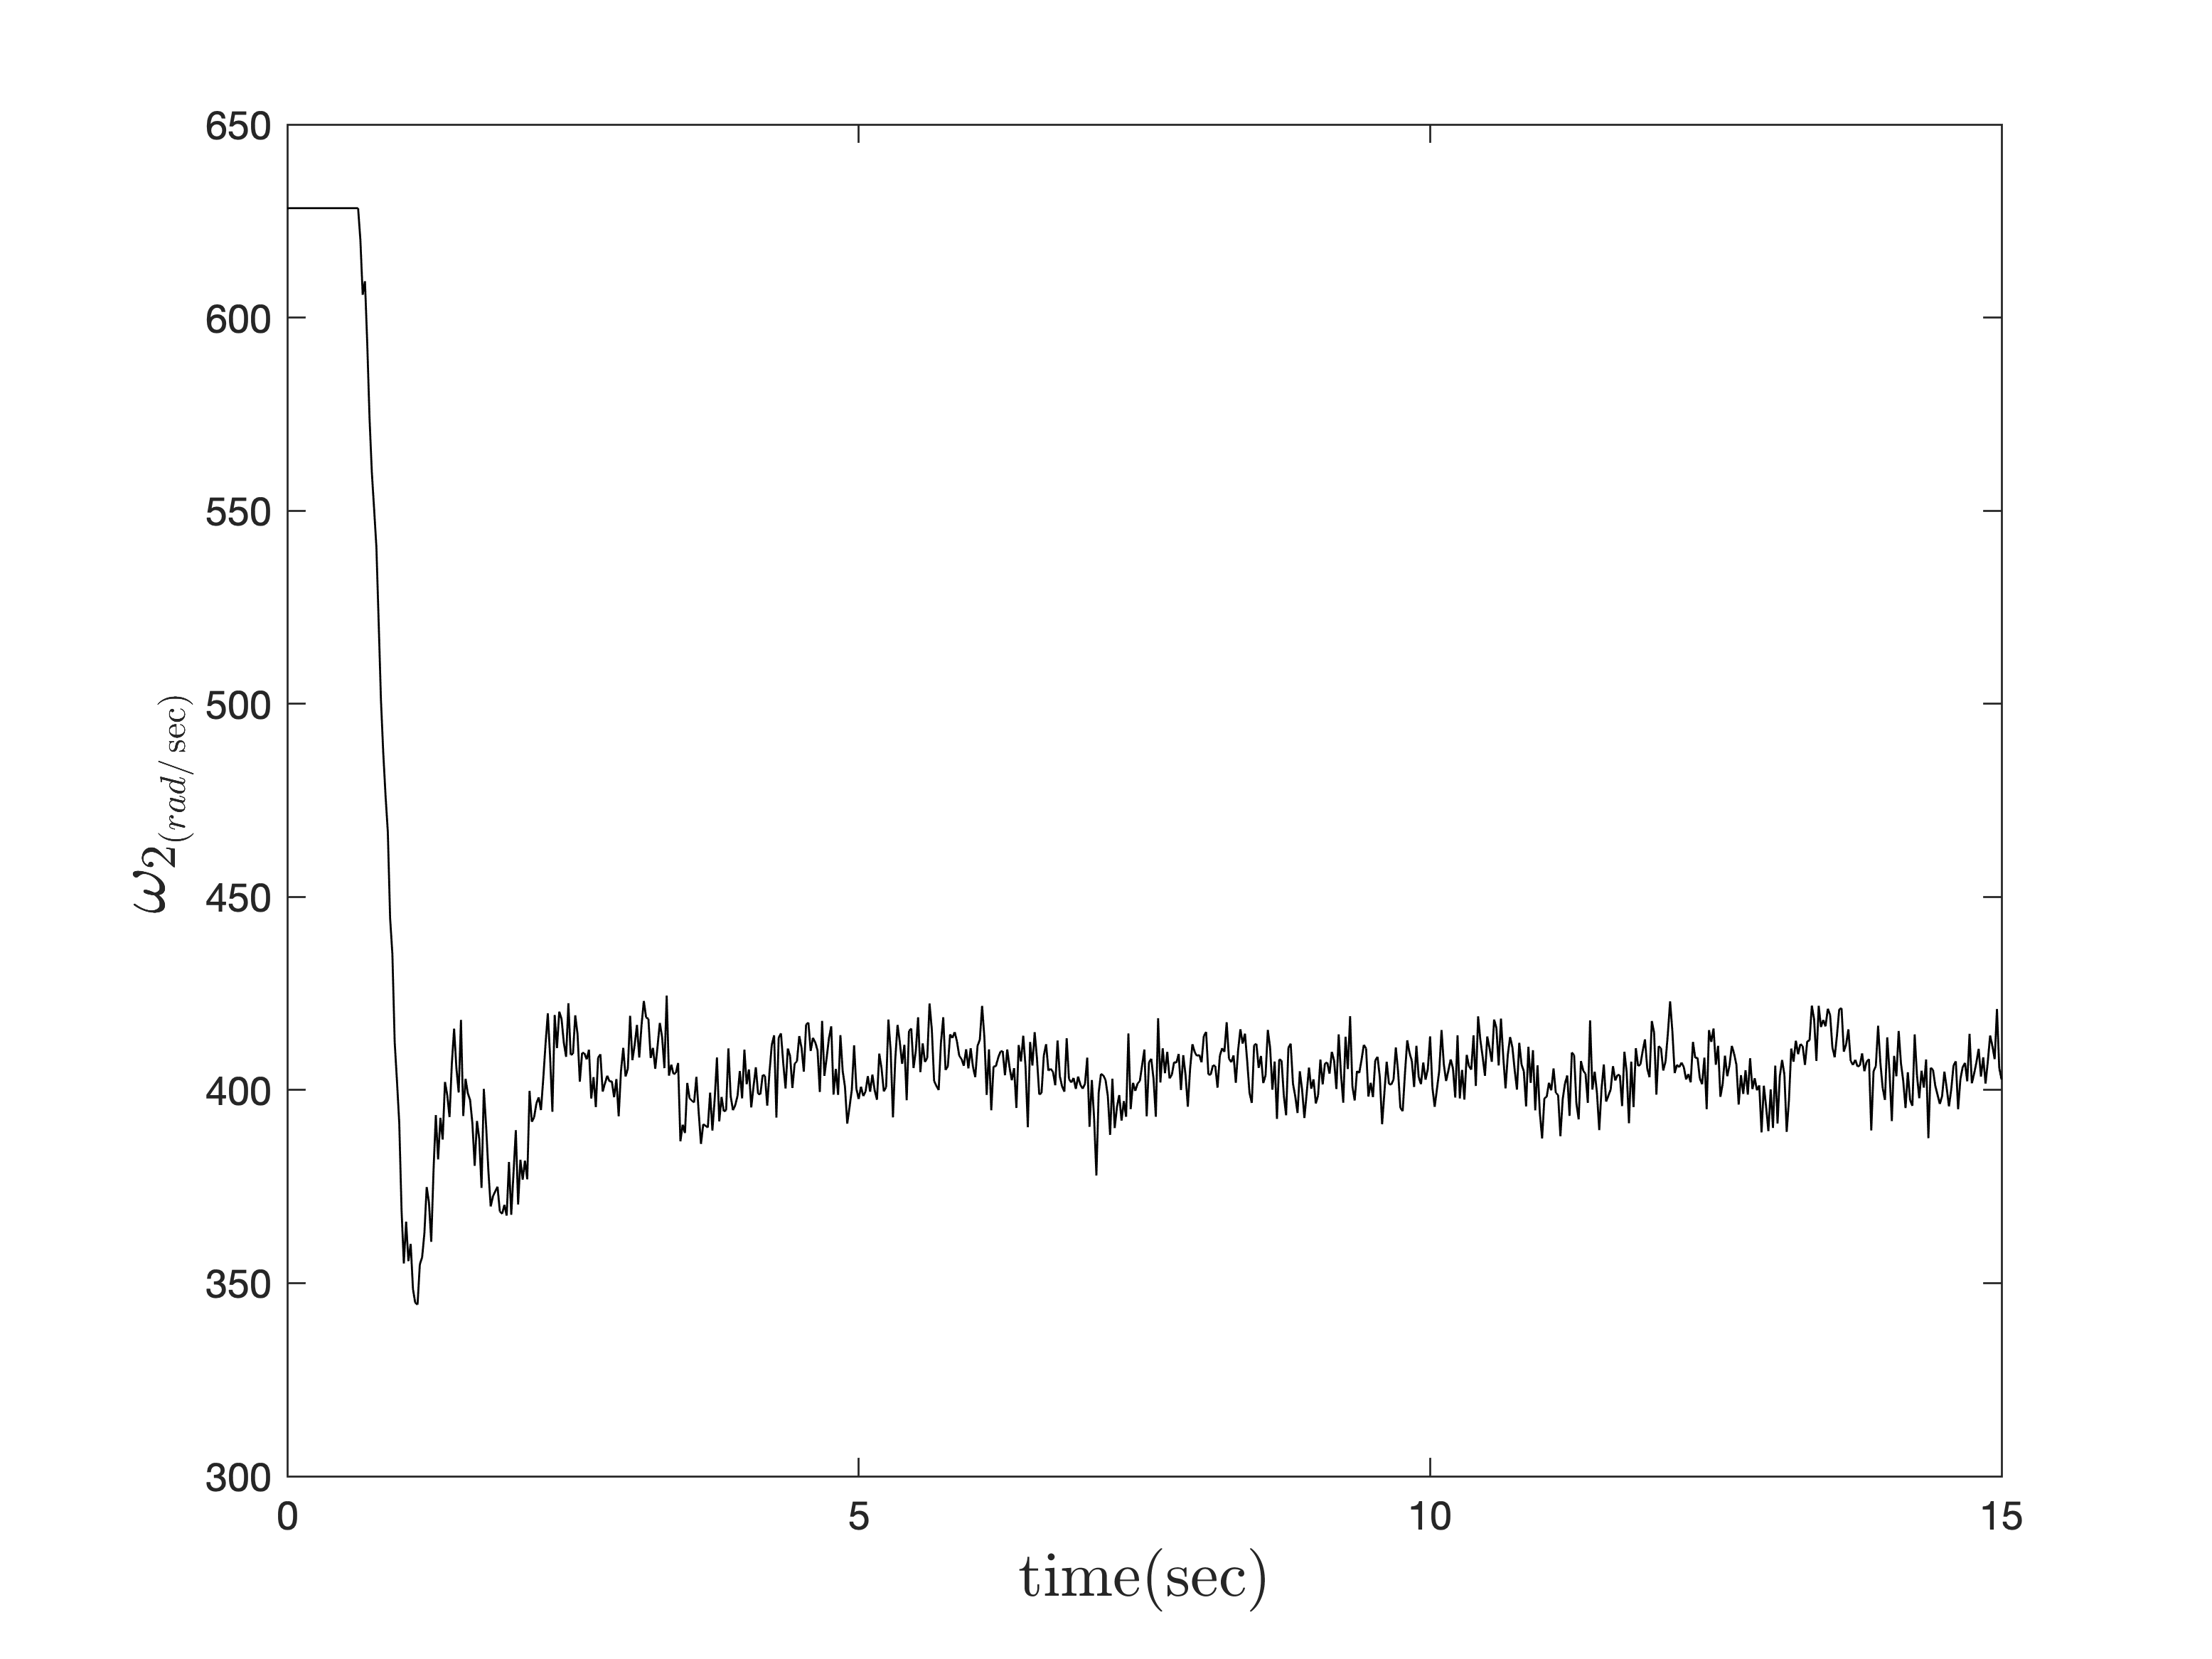
\includegraphics[width=.45\linewidth]{../Figures/MIL/LQIDG/3DOF/lqidg_roll_pitch_Omega_2.png}
	}
	\subfigure[موتور شماره سه]{
		\centering
		\includegraphics[width=.45\linewidth]{../Figures/MIL/LQIDG/3DOF/lqidg_roll_pitch_Omega_3.png}
	}
	\subfigure[موتور شماره چهار]{
		\centering
		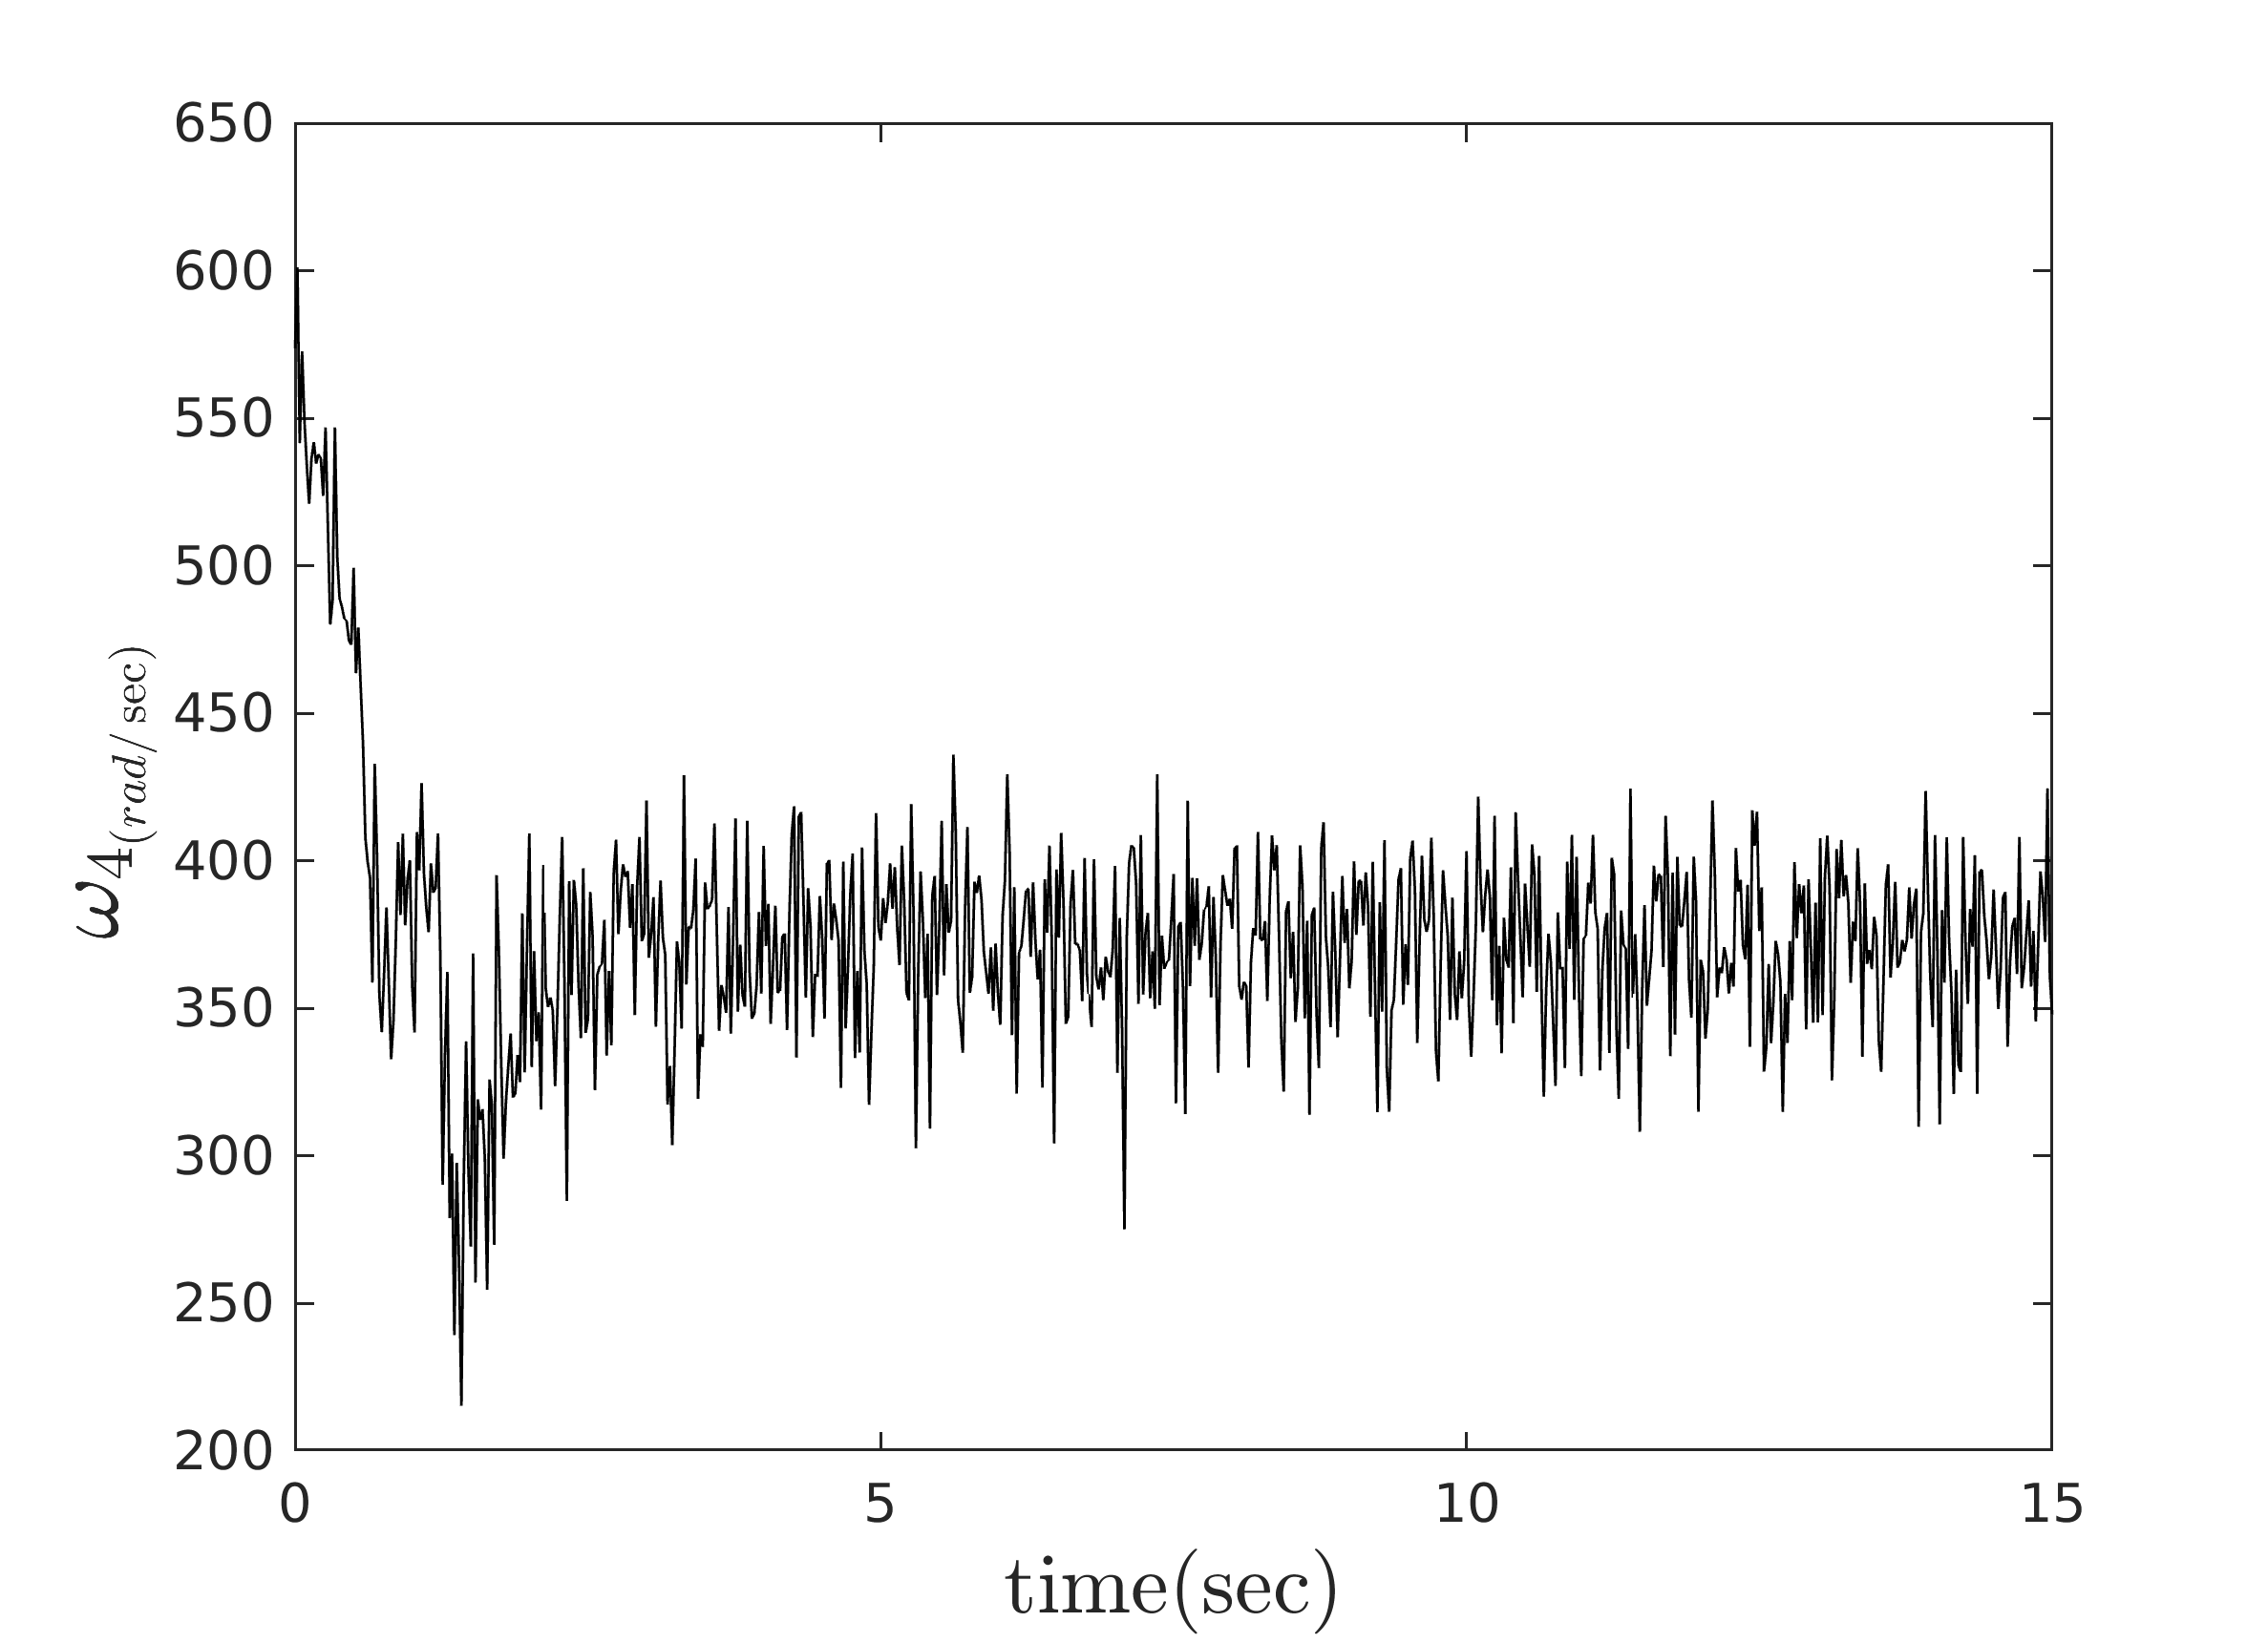
\includegraphics[width=.45\linewidth]{../Figures/MIL/LQIDG/3DOF/lqidg_roll_pitch_Omega_4.png}
	}
	\caption{‫‪فرمان کنترلی موتورها در کنترل زاویه رول، پیچ و یاو (تعقیب ورودی صفر)}
\end{figure}

\subsection{شبیه‌سازی کنترل‌کننده به‌صورت چهار ورودی}

%بر اساس خروجی شبیه‌سازی (شکل
%\ref{lqidg_roll_fig})
%،کانال رول در حضور کنترل‌کننده \lr{LQIDG} در حدود پنج ثانیه و کانال پیچ در حدود هشت ثانیه به تعادل می‌رسد و خطای ماندگار آن در حدود صفر است.

\begin{figure}[H]
	\centering
	\subfigure[تغییرات زاویه رول]{
		\centering
		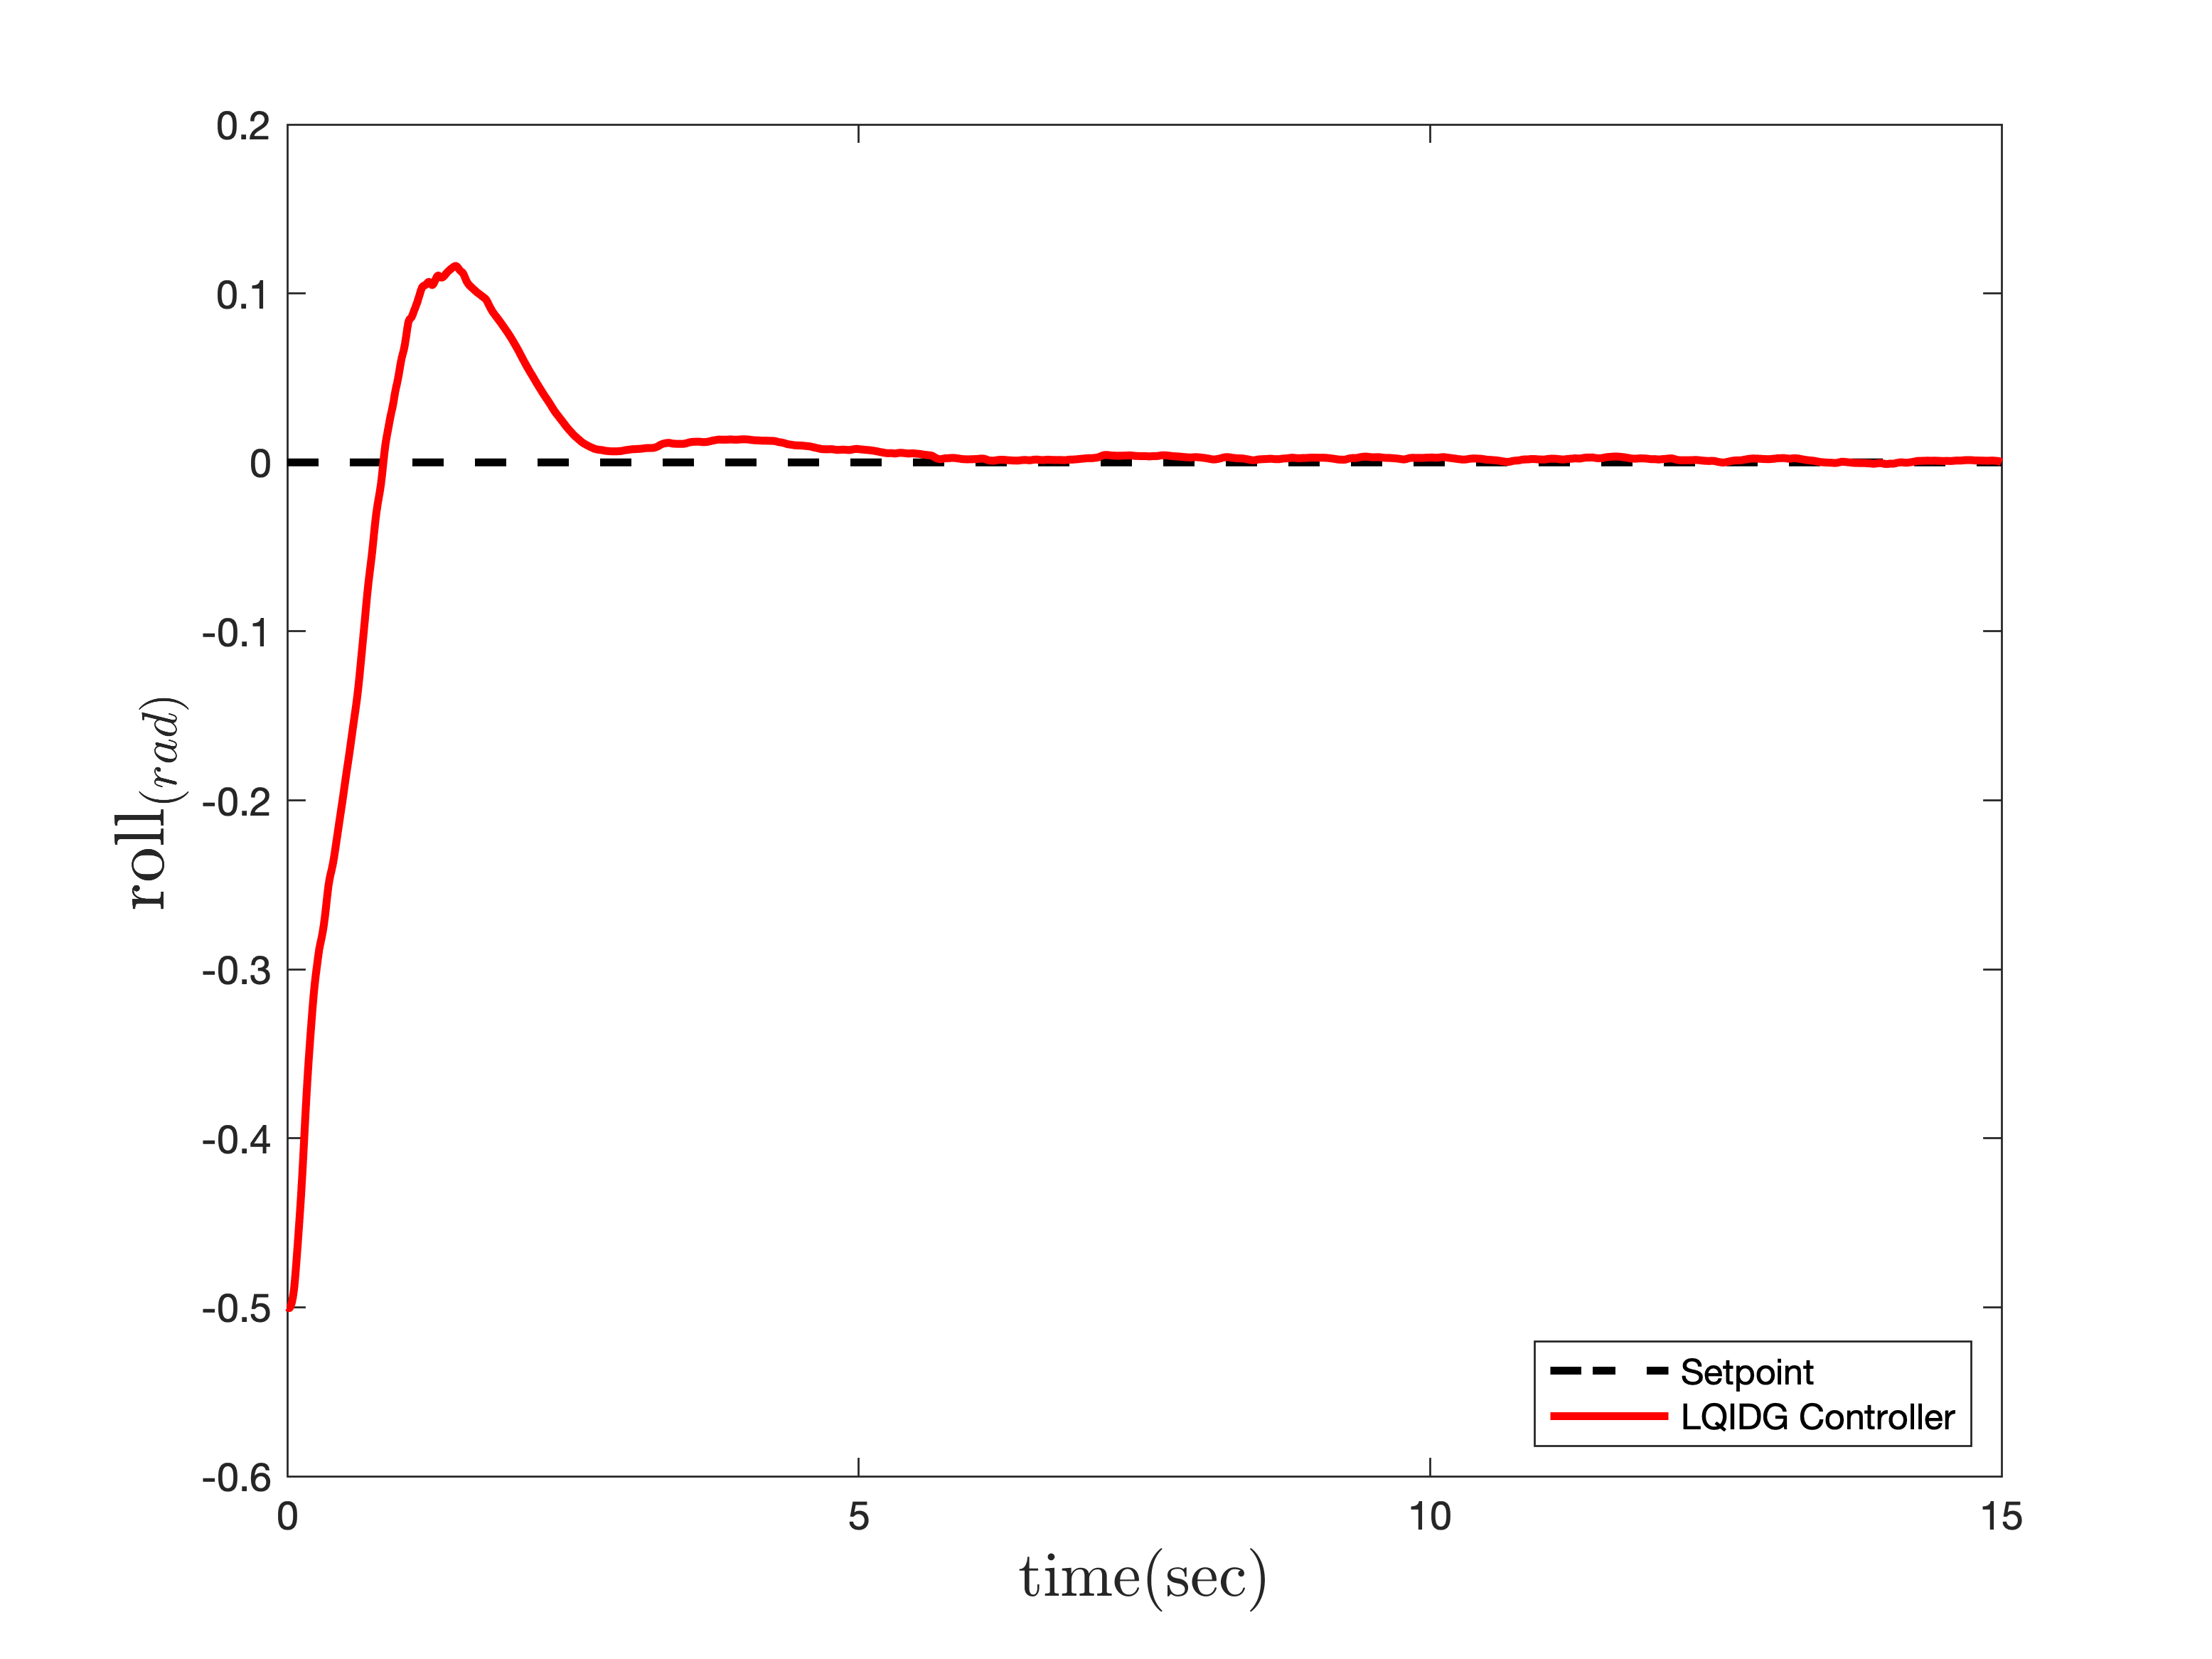
\includegraphics[width=.48\linewidth]{../Figures/MIL/LQIDG/MIMO/lqidg_roll.png}
	}
	\subfigure[تغییرات زاویه پیچ]{
		\centering
		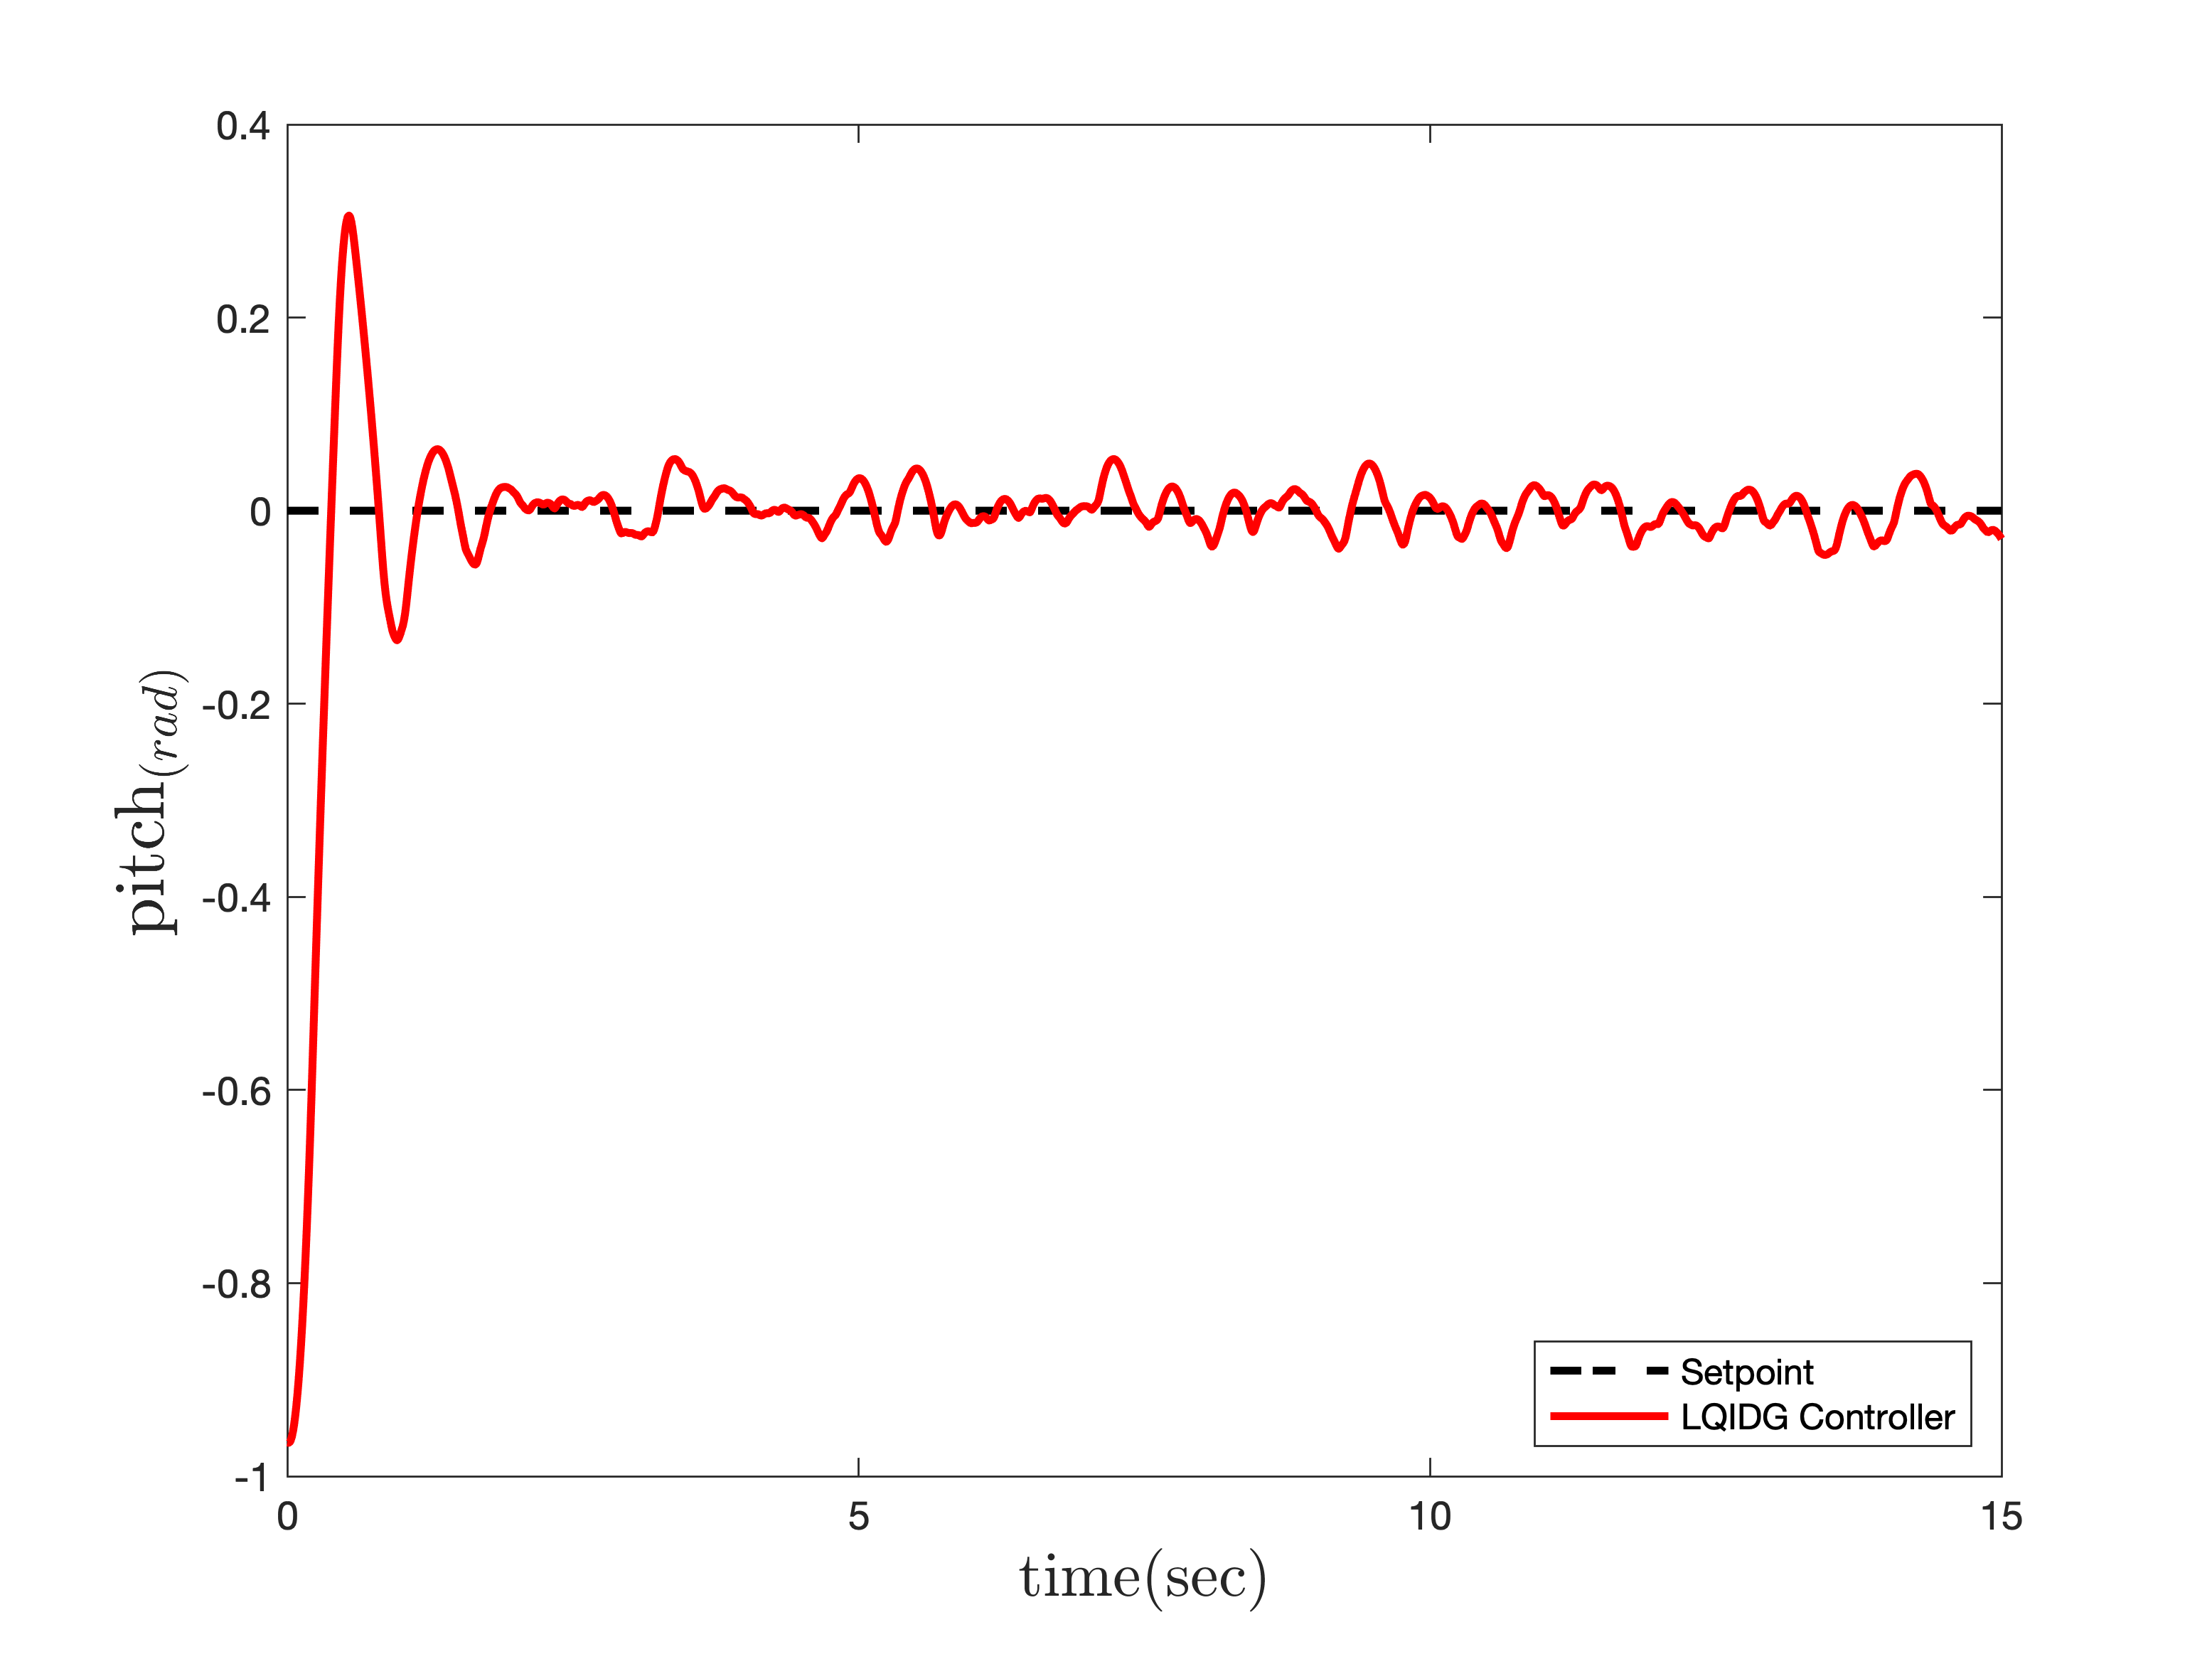
\includegraphics[width=.48\linewidth]{../Figures/MIL/LQIDG/MIMO/lqidg_pitch.png}
	}
	\subfigure[تغییرات زاویه یاو]{
		\centering
		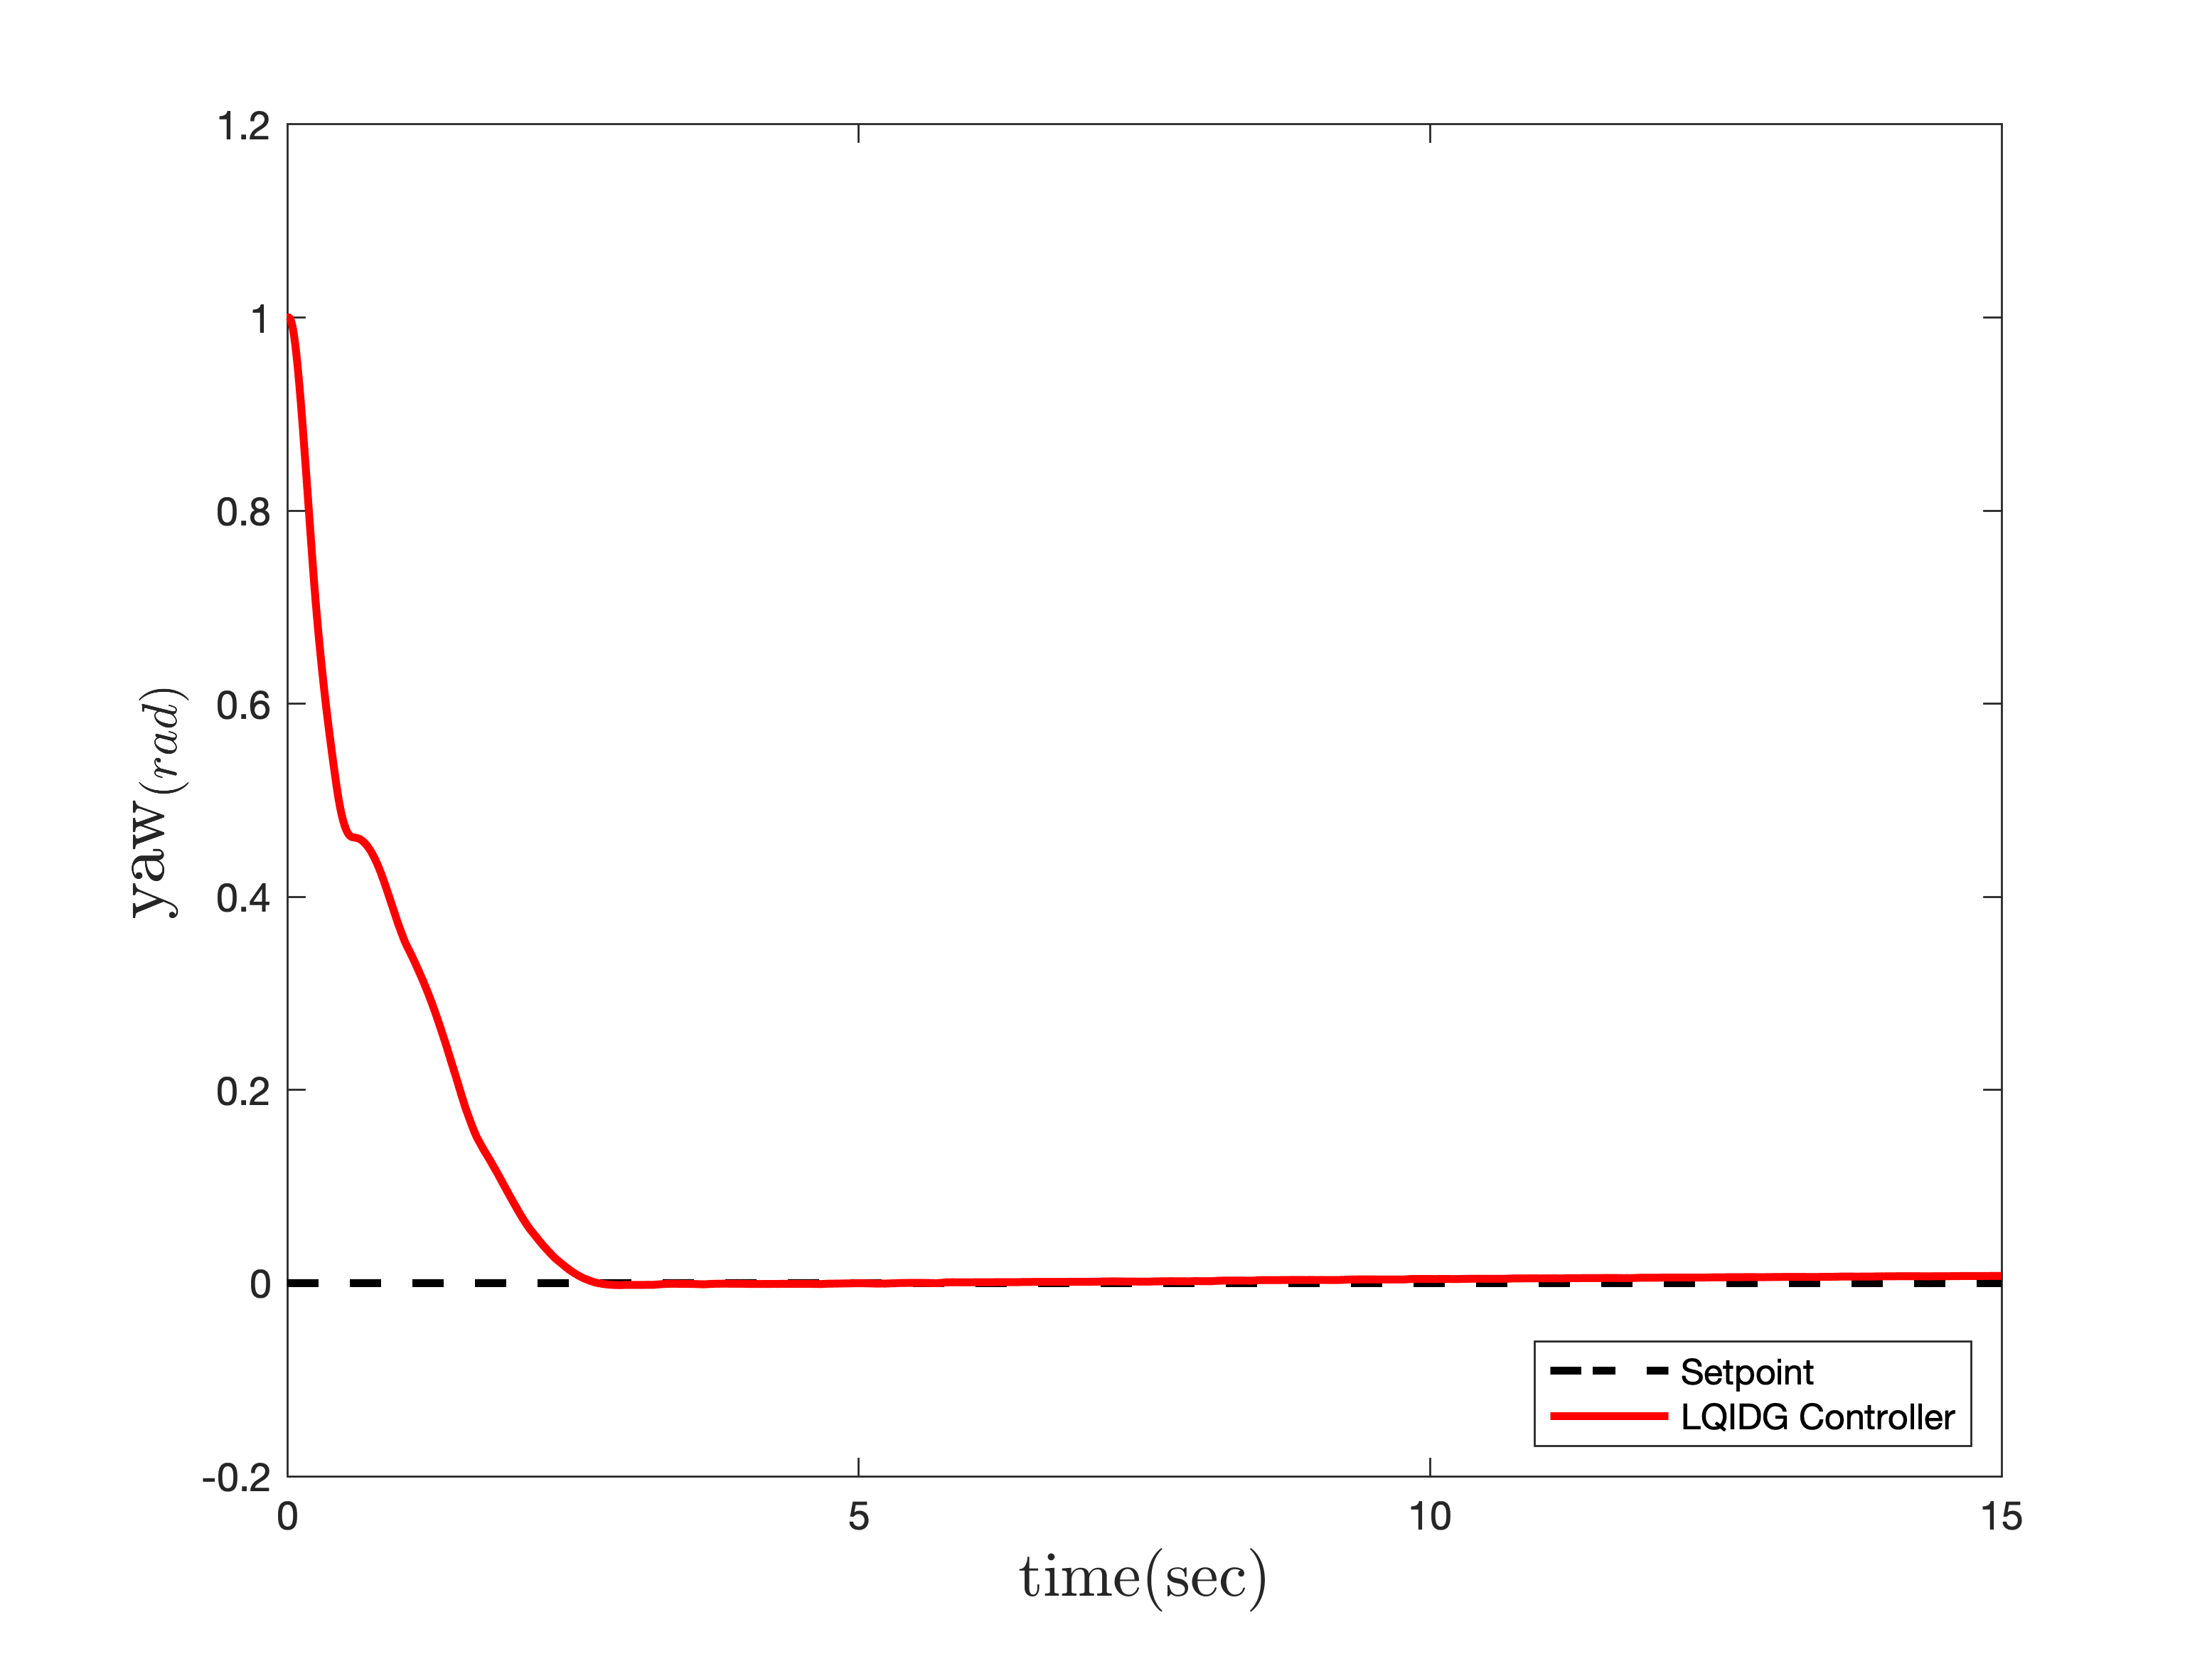
\includegraphics[width=.48\linewidth]{../Figures/MIL/LQIDG/MIMO/lqidg_yaw.png}
	}
	\caption{‫‪عملکرد کنترل‌کننده \lr{LQIDG} در کنترل زاویه رول، پیچ و یاو (تعقیب ورودی صفر)}
	\label{lqidg_roll_pitch_yaw_fig_simulation_MIMO}
\end{figure}


\begin{figure}[H]
	\centering
	\subfigure[موتور شماره یک]{
		\centering
		\includegraphics[width=.45\linewidth]{../Figures/MIL/LQIDG/MIMO/lqidg_roll_pitch_Omega_1.png}
	}
	\subfigure[موتور شماره دو]{
		\centering
		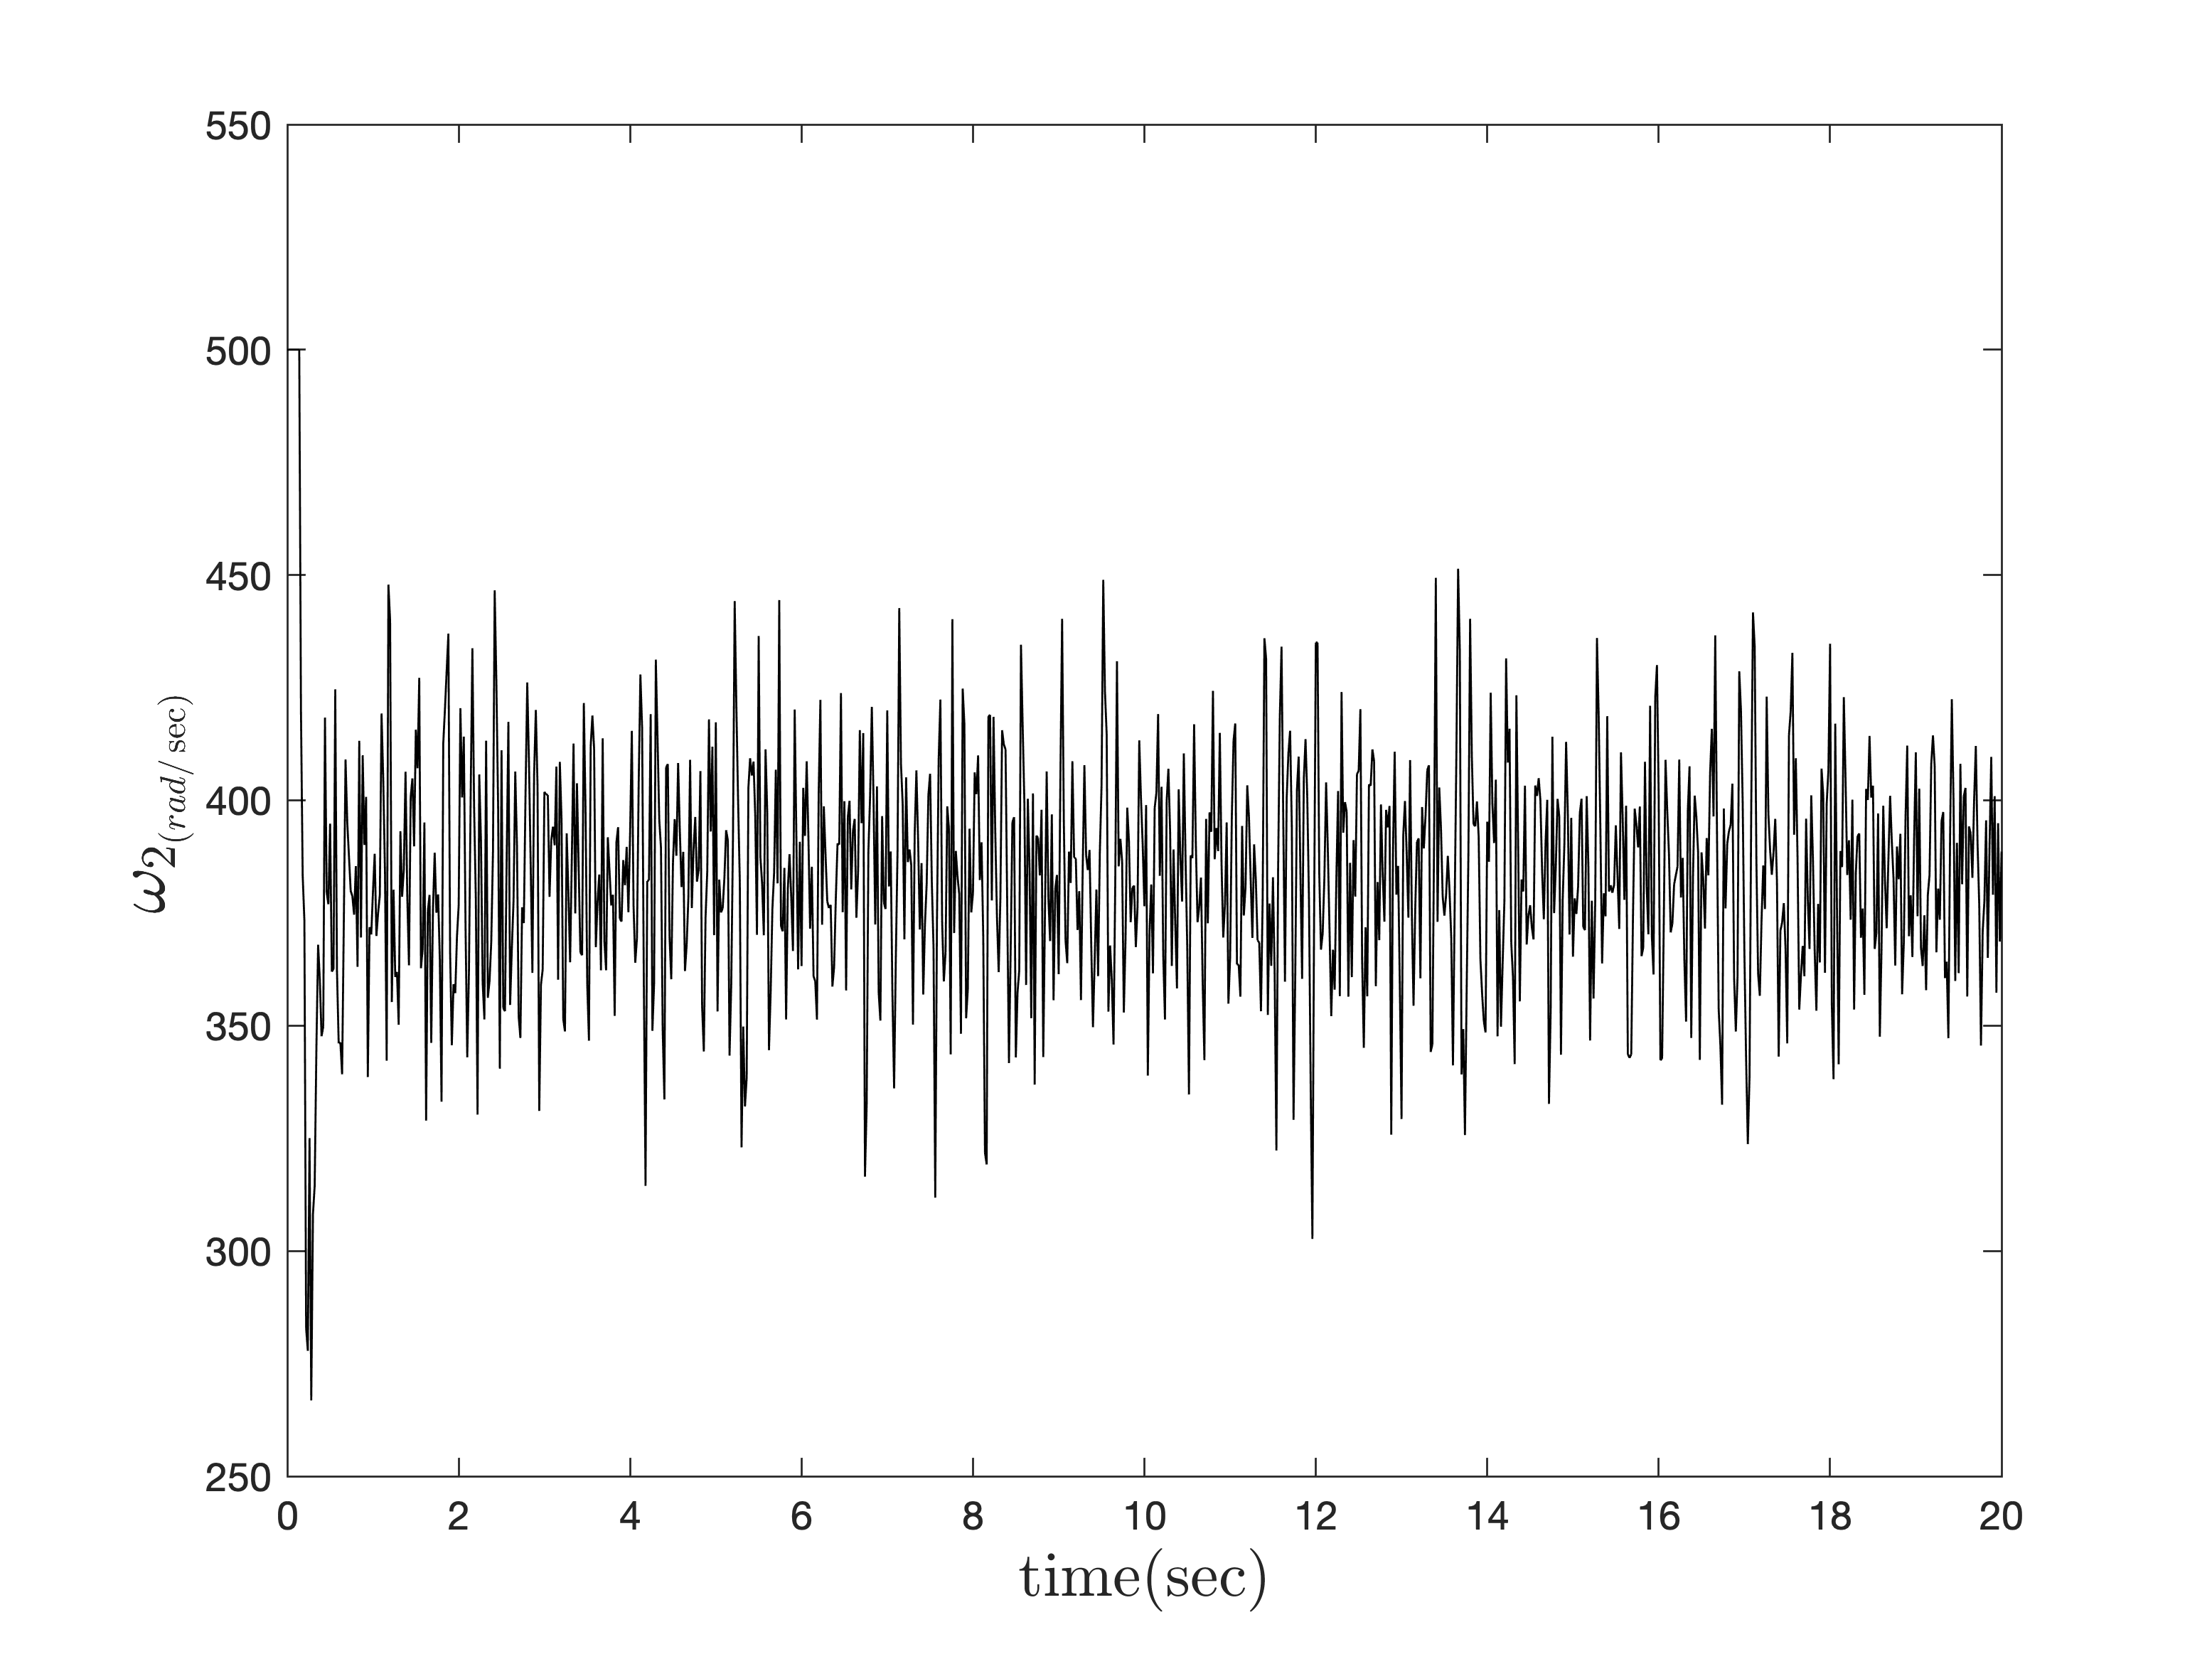
\includegraphics[width=.45\linewidth]{../Figures/MIL/LQIDG/MIMO/lqidg_roll_pitch_Omega_2.png}
	}
	\subfigure[موتور شماره سه]{
		\centering
		\includegraphics[width=.45\linewidth]{../Figures/MIL/LQIDG/MIMO/lqidg_roll_pitch_Omega_3.png}
	}
	\subfigure[موتور شماره چهار]{
		\centering
		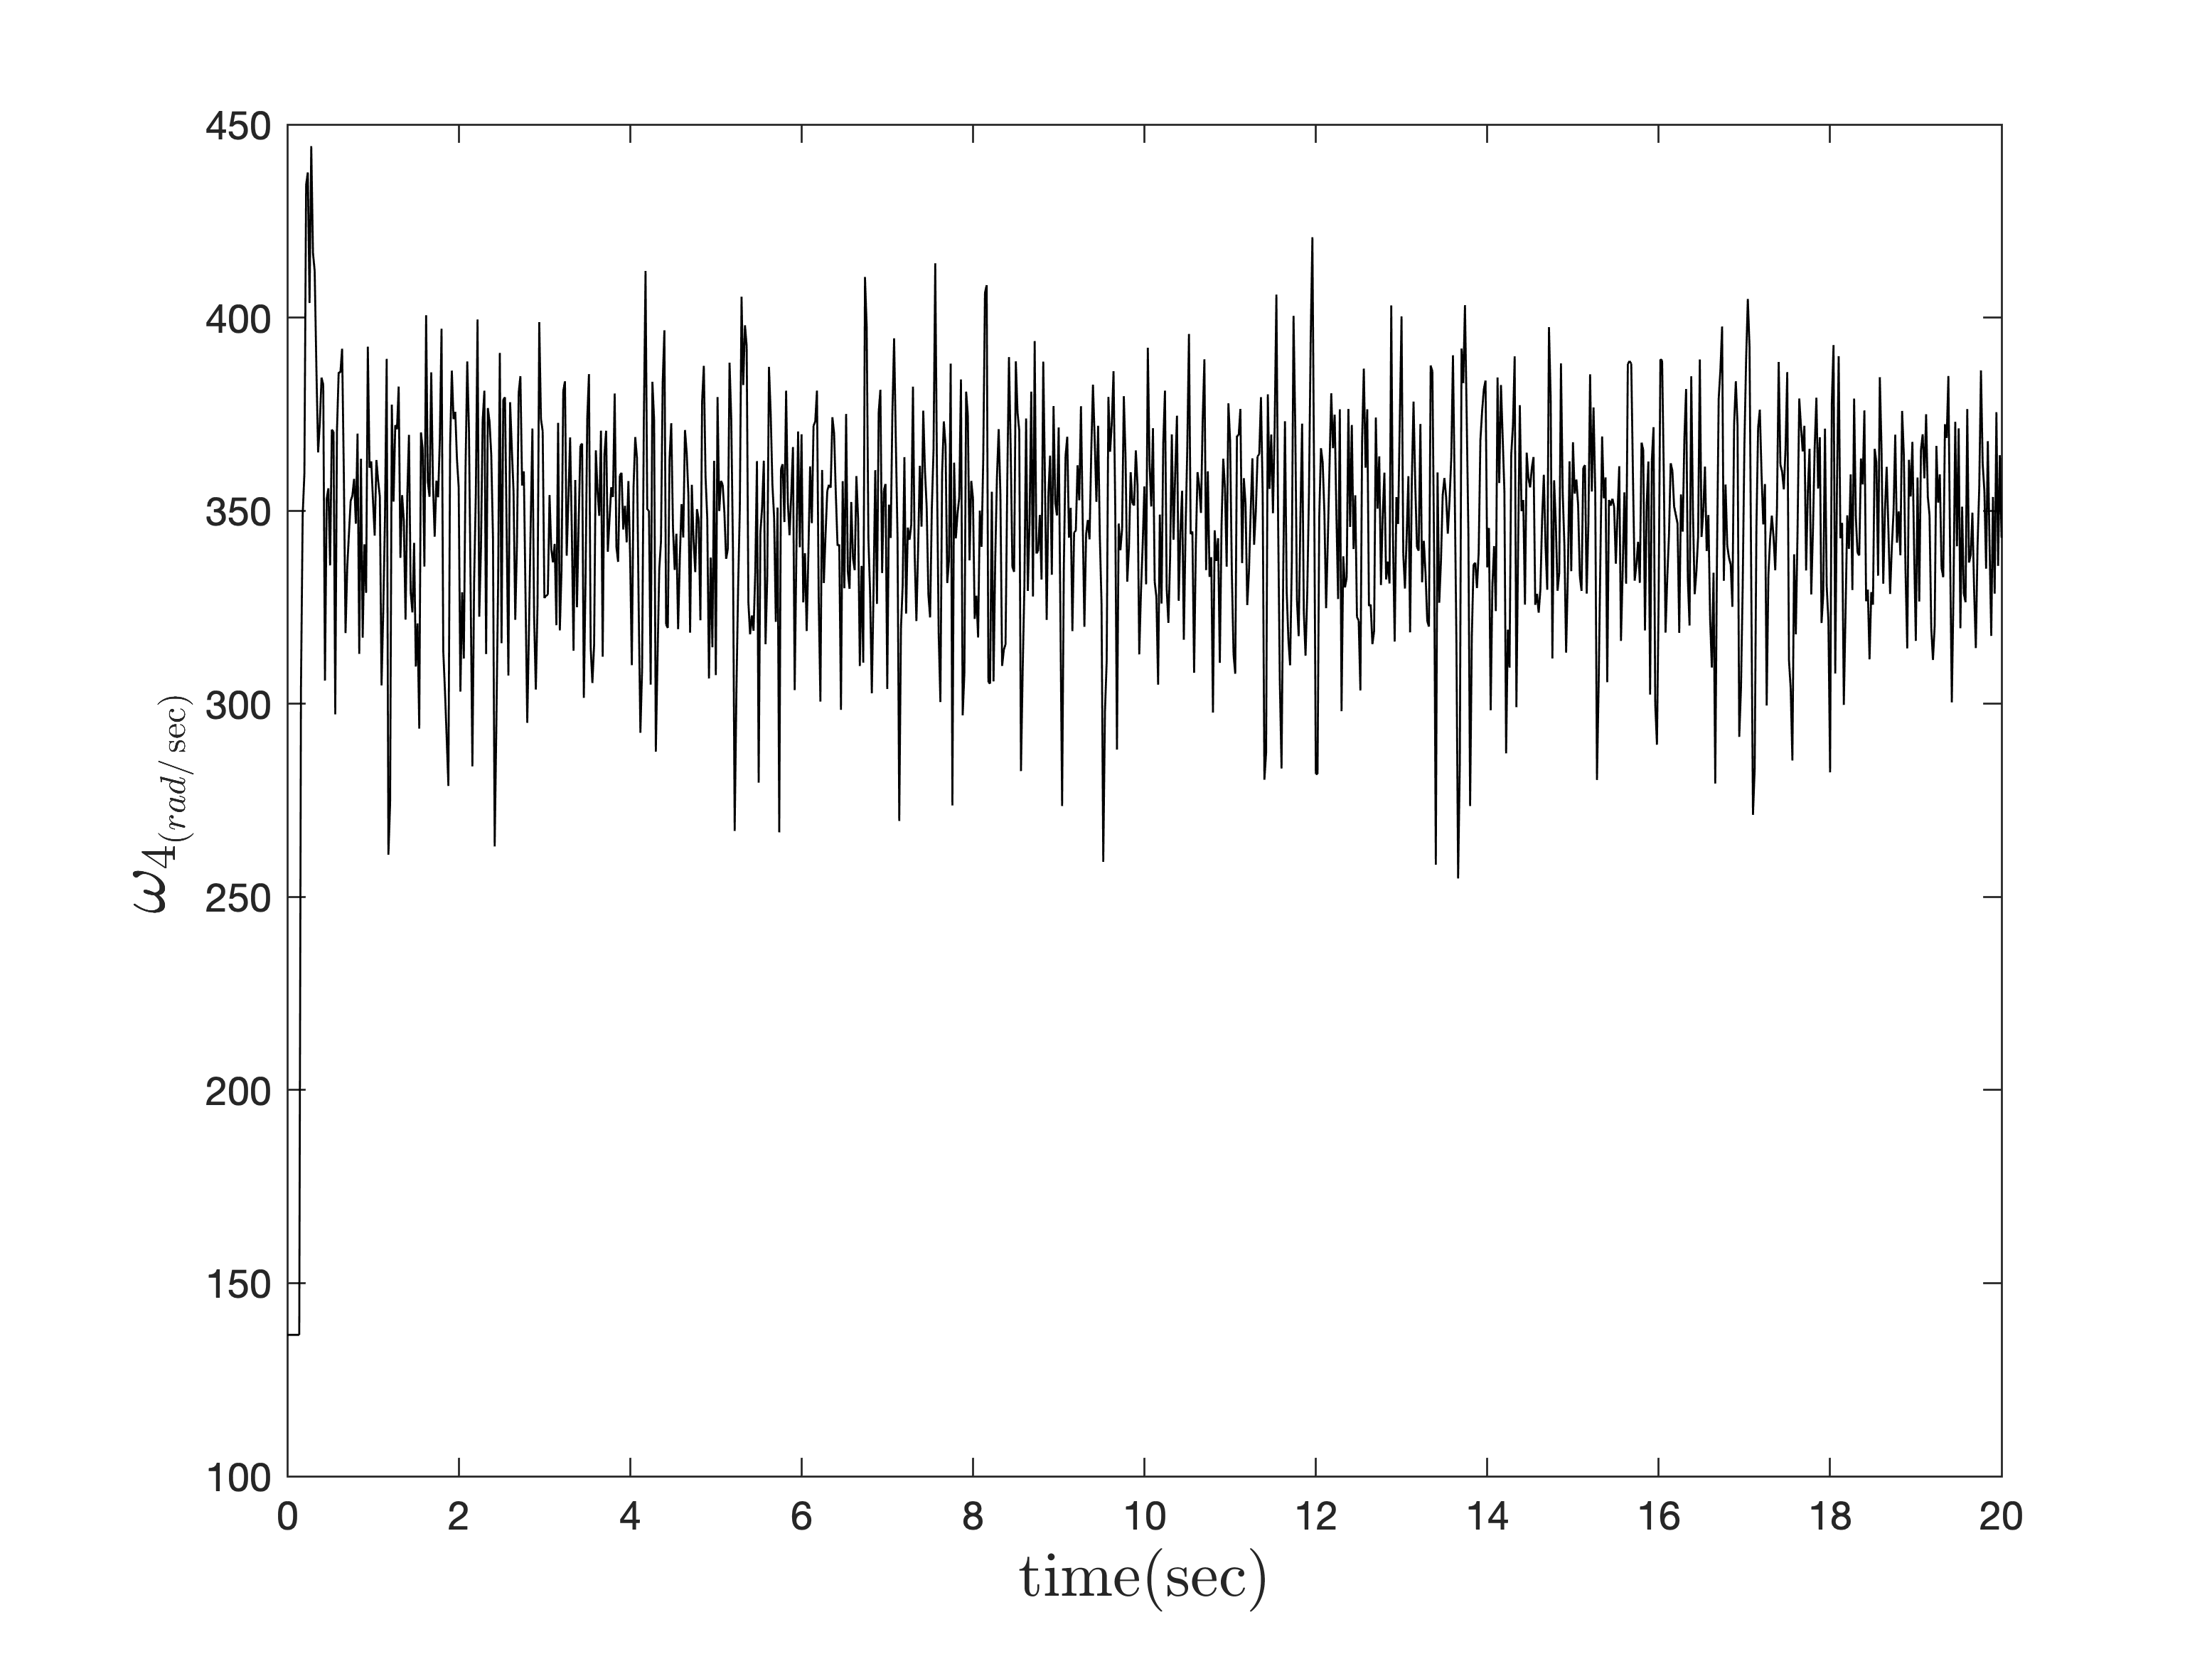
\includegraphics[width=.45\linewidth]{../Figures/MIL/LQIDG/MIMO/lqidg_roll_pitch_Omega_4.png}
	}
	\caption{‫‪فرمان کنترلی موتورها در کنترل زاویه رول، پیچ و یاو (تعقیب ورودی صفر)}
\end{figure}